% checks commands
\RequirePackage[l2tabu, orthodox]{nag}

% document class
\documentclass[12pt, letterpaper]{article}

% language
\usepackage[english]{babel}

% bibliography
\usepackage{natbib}

% math
\usepackage{amsmath, amsthm, amssymb, commath, cool}

% add notes
\usepackage[colorinlistoftodos, textsize = scriptsize, color = yellow!90]{todonotes}
\setlength{\marginparwidth}{1in}

% spacing
\usepackage{setspace}
\onehalfspacing

% margins
\usepackage[letterpaper, margin=1.2in]{geometry}

% nice tables
\usepackage{booktabs}
\usepackage{ctable}
\usepackage{tabularx} 
\usepackage{subcaption}

% table columns
\newcolumntype{C}{>{\centering\arraybackslash}X}

% pictures
\usepackage{graphicx}
\usepackage[toc,page]{appendix} % make appendix
\usepackage[pdftex, unicode, pdfauthor={Olga Rud}]{hyperref}
\hypersetup{colorlinks, citecolor=blue, filecolor=black, linkcolor=blue, urlcolor=blue}
\graphicspath{{figures/}}

% theorems
\theoremstyle{plain}

% math operatores
\DeclareMathOperator*{\argmax}{arg\,max}
\DeclareMathOperator*{\mex}{\mathbb{E}}
\DeclareMathOperator*{\ind}{\mathbb{I}}
\DeclareMathOperator*{\prob}{\mathbb{P}}

% spacing in notes
\newcommand{\smalltodo}[2][]
     {\todo[caption={#2}, #1]
     {\begin{spacing}{1}#2\end{spacing}}}

\begin{document}

\newtheorem{Assumption}{Assumption}
\newtheorem{Proposition}{Proposition}
\newtheorem{Corollary}{Corollary}
\newtheorem{Hypothesis}{Hypothesis}
\newtheorem{Result}{Result}


\title{An endogenous-timing conflict game}

\author{Youngseok Park 
\footnote{Korea Institute for International Economic Policy }  \and Jean Paul Rabanal
\thanks{Department of Banking and Finance, Monash University (Corresponding author)}
 \and Olga A. Rud \footnote{Department of Economics, RMIT Univeristy}  \and Philip J. Grossman\thanks{Department of Economics, Monash University } }
\date{\today}
\clearpage\maketitle
\thispagestyle{empty}

\begin{abstract}
\noindent We present an endogenous-timing conflict game of incomplete information under strategic complementarity. The model predicts multiple equilibria, in which the outcome follows either a simultaneous move game (Baliga and Sj\"ostr\"om, 2004) or a sequential game, which improves social welfare. We study the three families of games in the laboratory using gender-balanced sessions. Our results suggest that: (i) social welfare is higher in the endogenous-timing and sequential games compared to the simultaneous game; (ii) men and women make similar decisions in the simultaneous and sequential-move games; and (iii) in the endogenous-timing game women are less willing to commit to the risky action.

\end{abstract}
\textbf{Keywords:}
Conflict game; Endogenous timing; Gender; Laboratory experiment; Type uncertainty \\
\textbf{JEL codes:} C72, C92, D74, D82, D91
\newpage
\section{Introduction}
\label{sec:intro}

Coordination is an important element in many strategic interactions. In banking, for example, people may hoard cash not because they need to do so, but rather due to a belief that others will do so, thus leading to a self-fulfilling crisis, characterized by liquidity shortages. At the international level, a state may build up its supply of weapons to serve as a deterrent, which may compel their neighboring states to do so as well, thus leading to an arms race. Formally, this sort of strategic interactions is schematized as \textit{strategic complementarities}, in which a player's action choice positively depends on the probability that the opponent chooses the same action. Strategic complementarities have been studied in a wide range of applications including oligopoly (Farrell and Saloner, 1985), liquidity crises (Morris and Shin, 1998), and conflicts (Baliga and Sj\"ostr\"om, 2004, hereafter BS04).

We build on the original BS04 game in which players simultaneously choose either a dovish action ($D$) or a hawkish action ($H$) in an environment of incomplete information about their countertparty's player type. The action space can be characterized as (i) \textit{dominant strategy hawks}, those who will always play $H$ regardless of the opponent's action, (ii) \textit{dominant strategy doves}, those who will always play $D$ regardless of the opponent's action, and (iii) \textit{complementary types}, those who prefer to match actions with the opponent. While $DD$ is the Pareto optimal outcome, a complementary type player's fear that a counterparty may play $H$, due to not knowing their type, can trigger an escalating spiral of aggression and lead to a mutually destructive outcome. BS04 propose a Bayesian Nash Equilibrium (BNE) for the simultaneous move game (CGO) which suggests that complementary types at or below a unique cutoff point will play $D$, while those above the cutoff point will play $H$.

In this paper, we make two contributions to the conflict game literature. First, we refashion the CGO environment and introduce two new games to study precommitment in a conflict game that can enhance social welfare. We introduce a sequential move game (CGS), in which the order of play is exogenously imposed, and an endogenous-timing game (CGE), in which players can self-select the order of play. In the CGE game, in addition to the CGO equilibrium, we propose a separating equilibrium, in which the spiral of aggression is mitigated by early commitment to $D$. In the separating equilibrium, players self-sort such that the dovish types move first, and the hawkish types move second. Thus, the likelihood of the destructive outcome ($HH$) is lower than in CGO game, and social welfare is enhanced. To test the theoretical predictions of the three families of games (CGO, CGS, and CGE) we conduct a gender-balanced laboratory experiment and elicit cutoff strategies using a slider,\footnote{In our experimental design, we directly elicit cutoff strategies which allows us to observe a significant heterogeneity of choices, as described in Duffy and Ochs (2012) and, recently, Van Huyck et al. (2018).  For an overview of experiments on conflict and contest games, see Kimbrough et al. (2017). } which results in a rich distribution of choices across treatments. 

Second, we offer some exploratory evidence on the existence of gender differences in strategies in conflict games.  According to Simpson (2003) and Kuwabara (2005), in some simultaneous move games, such as Prisoner's Dilemma, different motivations across gender can lead to the same choices, and a subsequent conclusion of no gender difference. In particular, Simpson (2003) and Kuwabara (2005) argue that in a PD game, men defect due to greed and free riding, while women are motivated by fear and defect to avoid exploitation. Thus, in our CGO game one would expect that both genders will play $H$ but for different reasons. Men will play $H$ to exploit the gains, while women will play $H$ to avoid being exploited by greedy partners. The CGS game reduces, though does not eliminate, the fear of exploitation as there is always a chance that the counterparty is a dominant hawkish type, which results in similar behavior across genders. In the CGE game, there is uncertainty about whether the encounter will be simultaneous or sequential in nature. Fear can trigger a cutoff similar to the one predicted in the CGO game. However, payoff dominance can lead to cutoff choices which resemble the predictions of the CGS game. Varying the timing of play may help us exploit how uncertainty affects motivations of each gender, and whether timing in games is important for achieving Pareto superior outcomes.

Following previous lab experiments that also study BS04 (Khan, 2017 and Evdokimov and Garfagnini, 2018), we observe a higher frequency of $DD$ in the CGO game than predicted by BNE. In the CGS game, theory suggests that the cutoff strategy should increase the frequency of $DD$. Our experimental results confirm the direction of the predictions. Players adjust their cutoffs to play $D$ more often in the CGS treatment relative to the CGO treatment, but not to the extent predicted by theory under the assumption of risk neutrality. In the CGE treatment, the experimental results show that the social welfare is higher compared to the CGO game.

We do not find any statistical differences in the distributions of cutoffs across gender within the CGO and CGS treatments. Thus, the results are consistent with the fear/greed arguments that predict similar behavior across gender in the simultaneous move game. For the CGS game, exploitation is harder to achieve under the current parameterization unless a subject is a dominant hawkish type, so both genders adjust their cutoffs in the direction of the NE prediction. Lastly, in the CGE game, gender plays an important role in how the game is viewed: as a CGO or a CGS game. Our results suggest that fear triggers a cutoff similar to the one predicted in the CGO game for women, while payoff dominance may help explain the higher cutoff observed for men, which is also similar to the one observed in the CGS game. Men are more willing to set the stage and play $D$ in the first period, which incentivizes the second mover to follow, thus increasing social welfare. 



\section{Related literature}

The most closely related paper to our work is by Heggedal et al. (2018), who test the main predictions of Farrell and Saloner (1985) on the role of precommitment. In stage one, players simultaneously decide whether to (i) remain at status quo (known payoff), or (ii) choose an alternative (risky payoff) which is irreversible. In stage two, only those players who have not yet committed to an action choose between the two alternatives. If no player commits to an action in stage one, then second stage decisions become simultaneous. The results show that, when the risk of failure is low, players are willing to commit and that they follow the equilibrium cutoff strategy. When the risk of failure is high (i.e., a large payoff loss if the others do not follow through) players are less willing to commit and the behavior deviates from the theoretical prediction. These findings are similar to what we observe in our CGS treatment and partially, in our CGE treatment. In our experimental design, we are primarily interested in analyzing the type of behavior that prevails in CGE, relative to the CGO and CGS games.

The literature on global games, which studies outcomes when players are uncertain about a common fundamental, differs from our theoretical framework, but we consider it important to discuss here given the strategic complementarity of these games. For example, Brindisi et al. (2014) find that in an investment game endogenous timing improves social welfare. Their results indicate that while coordination is higher under endogenous timing, it is still lower than predicted. In the simultaneous-move game, subjects use a cutoff strategy which deviates from theory, and approaches payoff dominance. Other games of incomplete information (Van Huyck et al., 2018) and complete information (Heinemann et al., 2004 and Duffy and Ochs, 2012) also report similar findings. However, for some classes of simultaneous-move games of incomplete information, risk dominance becomes an important factor in strategy selection (Cabrales et al., 2007).

Gender may also play an important role in games of strategic complementarity. In a bank run experiment, Dijk (2017) reports that women are more likely to withdraw as fear increases, while Kiss et al. (2014) do not find significant differences on withdrawing rates across gender. The fear of being the ``sucker" may also impede cooperation (see Ingram and Berger, 1977; Van den Assem et al., 2012, and a recent lab-in-the-field experiment in rural India by Gangadharan et al., 2019). However, according to Babcock et al. (2017) women can overcome the ``sucker" effect in a dynamic volunteer game with strategic substitutes. Their findings suggest that when there is less payoff uncertainty, women volunteer more often than men, and thus improve social welfare. However, in our game of strategic complements, resolving the payoff uncertainty by playing $H$ does not lead to a Pareto superior outcome and, in fact, makes the CGE game resemble CGO. 


\section{The environment}
\label{sec:model}
The model builds on the simultaneous-move two-player conflict game of BS04. In this game of incomplete information, player $i$ can pursue either a hawkish (aggressive) action ($H$), or a dovish (peaceful) action ($D$). The action space for a player can be specified as $s\in\{H,D\}$, and leads to the following payoff matrix,

\begin{table}[h]
\centering
\caption{The conflict game}
\label{table:payoff}
\begin{tabular}{c|cc}
    & $H$ & $D$ \\ \hline
$H$ & $x_i, x_j$    & $\mu+x_i, k-d$     \\
$D$ &  $k-d, \mu+x_j$   & $k,k$
\end{tabular}
\end{table}
where $d<k$, and $\mu<d$ ($\mu > d$) when the game has strategic complements (substitutes). For completeness, we also present the game under strategic substitutes, though our main interest remains the case of strategic complements. When both players play $H$, player $i$ ($j$) receives $x_i$ ($x_j$), which is an idiosyncratic payoff that is independently drawn from a uniform distribution $F\in [0,k]$. Therefore, $x$ can be thought of as hawk type, in which some players are revealed to be more hawkish and thus reap more benefit from action $H$, and some are revealed to be less hawkish and see a lower return to playing $H$. If both players choose the dovish action $D$, then the payoff to each player is a constant $k$. If player $i$ plays $D$, while player $j\neq i$ plays $H$, then the payoff to player $i$ is $k-d>0$, where $d$ can be considered a cost of a dovish action when the opponent is hawkish. On the other hand, if player $i$ plays $H$ and player $j\neq i$ plays $D$, then the payoff to player $i$ is $\mu+x_i$, where $\mu>0$ can be viewed as a marginal benefit of an aggressive action when the opponent is dovish. 

The Bayesian Nash Equilibrium (BNE) can be characterized as a cutoff strategy such that a player with a type lower than $x_i\leq\hat{x}_{_{CGO}}$ will play $D$, and $H$ otherwise.  When a player is indifferent between $H$ and $D$, we can find the cutoff as the unique fixed point where 

\begin{equation}
\hat{x}_{_{CGO}}:= k-d + (d-\mu) F(\hat{x}_{_{CGO}}). \label{eq:cgo}
\end{equation}


\newtheorem{lem}{Lemma}
\begin{lem}
In the unique Bayesian Nash equilibrium (BNE), the probability that player $i$ plays $D$ is $F(\hat{x}_{_{CGO}})$, where $\hat{x}_{_{CGO}}$ is the unique fixed point of the player's best response as specified by equation (\ref{eq:cgo}).
\end{lem}\par

In the game with strategic complements, the fear of encountering dominant strategy hawks triggers an escalating spiral of aggression, which in turn causes a subset of complementary types ($x_i \in (\hat{x}_{_{CGO}}, k-\mu)$) to choose $H$ in the BNE (see Figure \ref{fig:typespace}). Using the parameters of our experiment $\{k=100, \mu=10, d=95 \}$, the cutoff point can be rewritten as 
\begin{equation}
\hat{x}_{_{CGO}}:= \frac{k\cdot (k-d)}{k-d+\mu}=33. \label{eq:cgosol}
\end{equation}


\begin{center}
\begin{figure}[ht]
\centering{}%
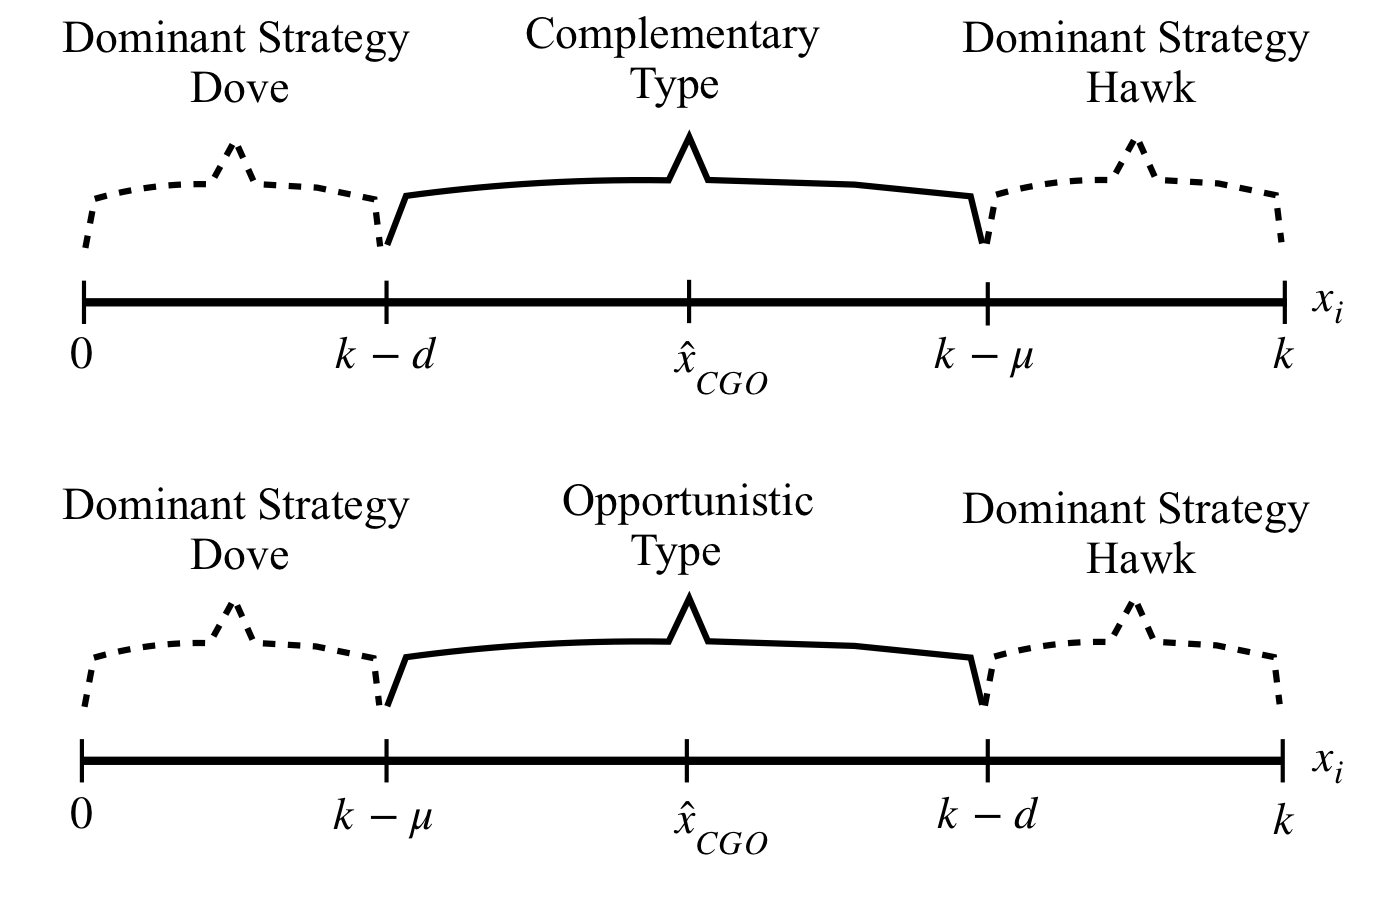
\includegraphics[scale=0.21]{typespace.jpg}%
\caption{Player type ($x_i$) space according to Table \ref{table:payoff} under strategic complements (top) and substitutes (bottom). $\hat{x}_{_{CGO}}$ is the BNE in the simultaneous game.} 
\label{fig:typespace}
\end{figure}
\end{center}

We examine whether the spiral of fear can be reduced by using strategic precommitment and varying the timing of play. A possible mechanism for improving welfare in a simultaneous-move game (CGO) with strategic complements is for players to move sequentially, in either an exogenous sequential-move game (CGS) and/or an endogenous-timing game (CGE). In the former, the order of play is randomly determined while in the latter players self-select the order of play. Social welfare under a CGS game is significantly higher relative to the CGO game. However, in a CGE game social welfare can be similar to either the CGO or a CGS environment, depending on the order of play selected by players. We begin by describing the optimal strategy in a CGS game, in which a player is randomly selected to move first after selecting their cutoff strategy. 

In the CGS game, the cutoff strategy for the first mover shifts to the right of the optimal strategy in the CGO game. The intuition for the rightward shift in the cutoff strategy is fairly straightforward. Consider a first mover whose type is complementary, $x_i \in (k-d, k-\mu)$, in Figure \ref{fig:typespace}. If the first mover selects $D$, then the second mover will play $D$ unless the second mover is a dominant strategy hawk. In other words, if the first player chooses $D$, the probability that the second player chooses $D$ is  $Pr(x_j\leq k-\mu) \equiv F(k-\mu)$, which is greater than $Pr(x_j\leq\hat{x}_{_{CGO}}) \equiv F(\hat{x}_{_{CGO}}$) in the CGO game. Therefore, the cutoff strategy for the first mover in a CGS game shifts to the right of the optimal strategy in a CGO game, such that $\hat{x}_{_{CGO}}\leq\hat{x}_{_{CGS}}$ when the game has strategic complements.

\begin{lem}
There exists a unique perfect Bayesian Nash equilibrium (PBNE) in which the first mover uses the cutoff strategy, $\sigma_i(x_i)=D$ if $x_i\leq \hat{x}_{_{CGS}} \equiv k-d\cdot(1-F(k-\mu))-\mu\cdot F(k-d)$.  In the PBNE, $\hat{x}_{_{CGO}}<\hat{x}_{_{CGS}}$ when the game has strategic complements and $\hat{x}_{_{CGO}}>\hat{x}_{_{CGS}}$ when the game has strategic substitutes.
\end{lem}\par
\noindent \textit{Proof:} See Appendix A $\blacksquare$

Using the parameters of our experiment, the unique PBNE in which the first mover uses the cutoff strategy can be defined as
\begin{equation}
\sigma_i(x_i)=D \quad \text{if} \ \ x_i\leq \hat{x}_{_{CGS}}:= k-\mu=90. 
\end{equation}

Next, we examine the CGE game in which players self-select the order of play. In this environment, after selecting their respective cutoffs, players simultaneously decide whether to move early or late. When a player decides to move early, the player commits to the action chosen during the cutoff stage. A player who chooses to move late is not constrained by the action specified in the cutoff stage.\footnote{Hamilton and Slutsky (1990) introduce this rule of endogenous timing in the form of the extended game with action commitment in a duopoly game under complete information.} Formally, the timing of the game proceeds as follows:

\textit{Stage 0:} Each player $i$ selects a cutoff strategy, indicating a set of values where $\sigma_i(x_i)=H$, and then observes own type $x_i$, but not the other player's type $x_j$ where $j\neq i$.

 \textit{Stage 1:} Both players simultaneously select the period in which to play the game $t=1,2$. 

\textit{Stage 2:} The conflict game is played by the move structure determined in Stage 1. The commitment to the cutoff strategy is not binding for player $i$ if and only if $t_i=2$ and $t_j=1$. 

The prediction for the cutoff strategy in the CGE game with strategic complements can follow either the CGO or CGS predictions. First, there exists a pooling equilibrium in which every type $x_i \in [0,k]$ selects the same period of play. In such case, the CGE game resembles the CGO game (Lemma 1). There also exists a separating equilibrium, in which a subset of types commit to an early dovish action ($t_{i}(x_i)=1; D$), while other types wait ($t_{i}(x_i)=2$). This separating equilibrium is consistent with Lemma 2. The results are summarized in Proposition 1.\footnote{Under a general distribution of $F(\cdot)$, there are in-between types ($x_i \in ( \hat{x}_{_{CGS}}, k-\mu)$) who exhibit a wait-and-see attitude. They are unwilling to commit early, but if the opponent commits to $D$, then they will reciprocate.}

\newtheorem{prop}{Proposition}
\begin{prop}
In the endogenous-timing conflict game there exists a pooling equilibrium  when the game is characterized by either strategic substitutes or complements. When the game is characterized solely by strategic complements, there exists a unique separating equilibrium, such that player strategies are defined as: $t_{i}(x_i)=1; D$ for $x_i\leq \hat{x}_{_{CGS}}$, and $t_{i}(x_i)=2$ for $x_i>\hat{x}_{_{CGS}}$. 

\end{prop}\par
\noindent \textit{Proof:} See Appendix A $\blacksquare$

\section{Hypotheses}

We draw our hypotheses for the family of games characterized by strategic complementarity, or $\mu<d$ in Table \ref{table:payoff}. \\

\noindent \textbf{Hypothesis 1}
\textit{In the simultaneous-move conflict game (CGO) subjects play at or above the cutoff strategy $\hat{x}_{_{CGO}}=33$.}\\

We reconcile the theoretical solution of the CGO game with experimental evidence for our first prediction. In the laboratory, subjects play $D$ more often than predicted by the Nash Equilibrium (NE). \\

\noindent \textbf{Hypothesis 2}
\textit{The cutoff strategy in the sequential-move CGS game is higher compared to the cutoff strategy in the simultaneous move CGO game.}\\

Note that the equilibrium predictions $\hat{x}_{_{CGS}}=90$ and $\hat{x}_{_{CGO}}=33$ are far apart. This allows us to observe meaningful differences even when players chose cutoff values greater than the NE described in Prediction 1. The gain in expected payoff is equal to $d\times \left( F(\hat{x}_{_{CGS}})-F(\hat{x}_{_{CGO}}) \right)=95\times( 90-33)/100=50$ points or 137\%. \\

\noindent \textbf{Hypothesis 3} \textit{In the CGE environment, there exist multiple equilibria which may lead to outcomes similar to either a CGO game or the CGS game.}\\

We propose an experiment to test which equilibrium, if any, will prevail under endogenous timing. \\

\noindent \textbf{Hypothesis 4} \textit{Social welfare, measured as joint profit, should be higher in the CGS game compared to the CGO game. In the CGE game, social welfare is at least as great as in the CGO game}.\\

Joint profit is higher when both parties select $DD$, which appears more frequently in the CGS game. The CGE game can lead to either a CGS game or CGO game. Thus, no matter what type of outcome prevails in the CGE game, we expect that social welfare is no smaller than in the CGO game.\\

\section{Laboratory procedures}
\label{sec:game}

The experiment was conducted at the Rosario Experimental and Behavioral Economics Lab (REBEL) of the Universidad del Rosario, Colombia. Participants were undergraduate students from all fields and were recruited online via ORSEE (Greiner, 2015). Subjects were part of one of the three treatments (between design): CGO, CGS and CGE,  with a session consisting of five practice periods and 11 paid periods. We paid subjects for all 11 periods.\footnote{For the documentation in Spanish, the language used for the sessions in Colombia, please contact the corresponding author.} Overall, we conducted nine sessions, with two silos per session. In each session there were two roughly gender-balanced silos of 12 subjects, each playing one of the three games. The subjects were not informed that the study also focused on analyzing possible gender differences.

In each silo, the game began with five solo practice rounds, in which the counterparty was a robot who played the NE prediction.\footnote{The motivation behind using a robot was to help subjects learn how a threshold strategy works in this environment. The robot used the same strategy in all treatments, to keep the effect of practice constant. There is no evidence that robot strategies affected actual play since players in the CGO game did not converge to the predicted NE (see Result 1). Furthermore, we do not mention in the instructions that the robot is using an optimal or equilibrium strategy.} The subject's task was to pick the minimum number of $x$ in the interval $[0,101]$ for which he/she will play $H$ (labelled $A$ in the experiment). That is, we directly ask the subject to select a cutoff strategy without having the knowledge of own $x$, and that of the counterparty. The user-interface designed in oTree (Chen, et al., 2016) is depicted in Figure \ref{fig:ui}. To select a cutoff value, the participant used a mouse to move the slider, and then confirmed her choice by clicking ``Next." For example, a subject who would like to play only $D$ ($H$) should move the slider to the extreme right (left). The user-interface in Figure \ref{fig:ui} presents the updated payoff matrix with the cutoff selection. In the payoff matrix, the unknown value of $x$ for the counterparty is depicted as $NN$.

Following five practice rounds, subjects played 11 paid rounds. Each subject was matched with another subject only once (perfect stranger matching).  In all three treatments, subjects selected their cutoffs simultaneously, and were unaware of their counterparty's gender. The steps following the cutoff selection varied according to treatment. We summarize the variations of the game in Table \ref{table:time}. 

\begin{center}
\begin{figure}[ht]
\centering{}%
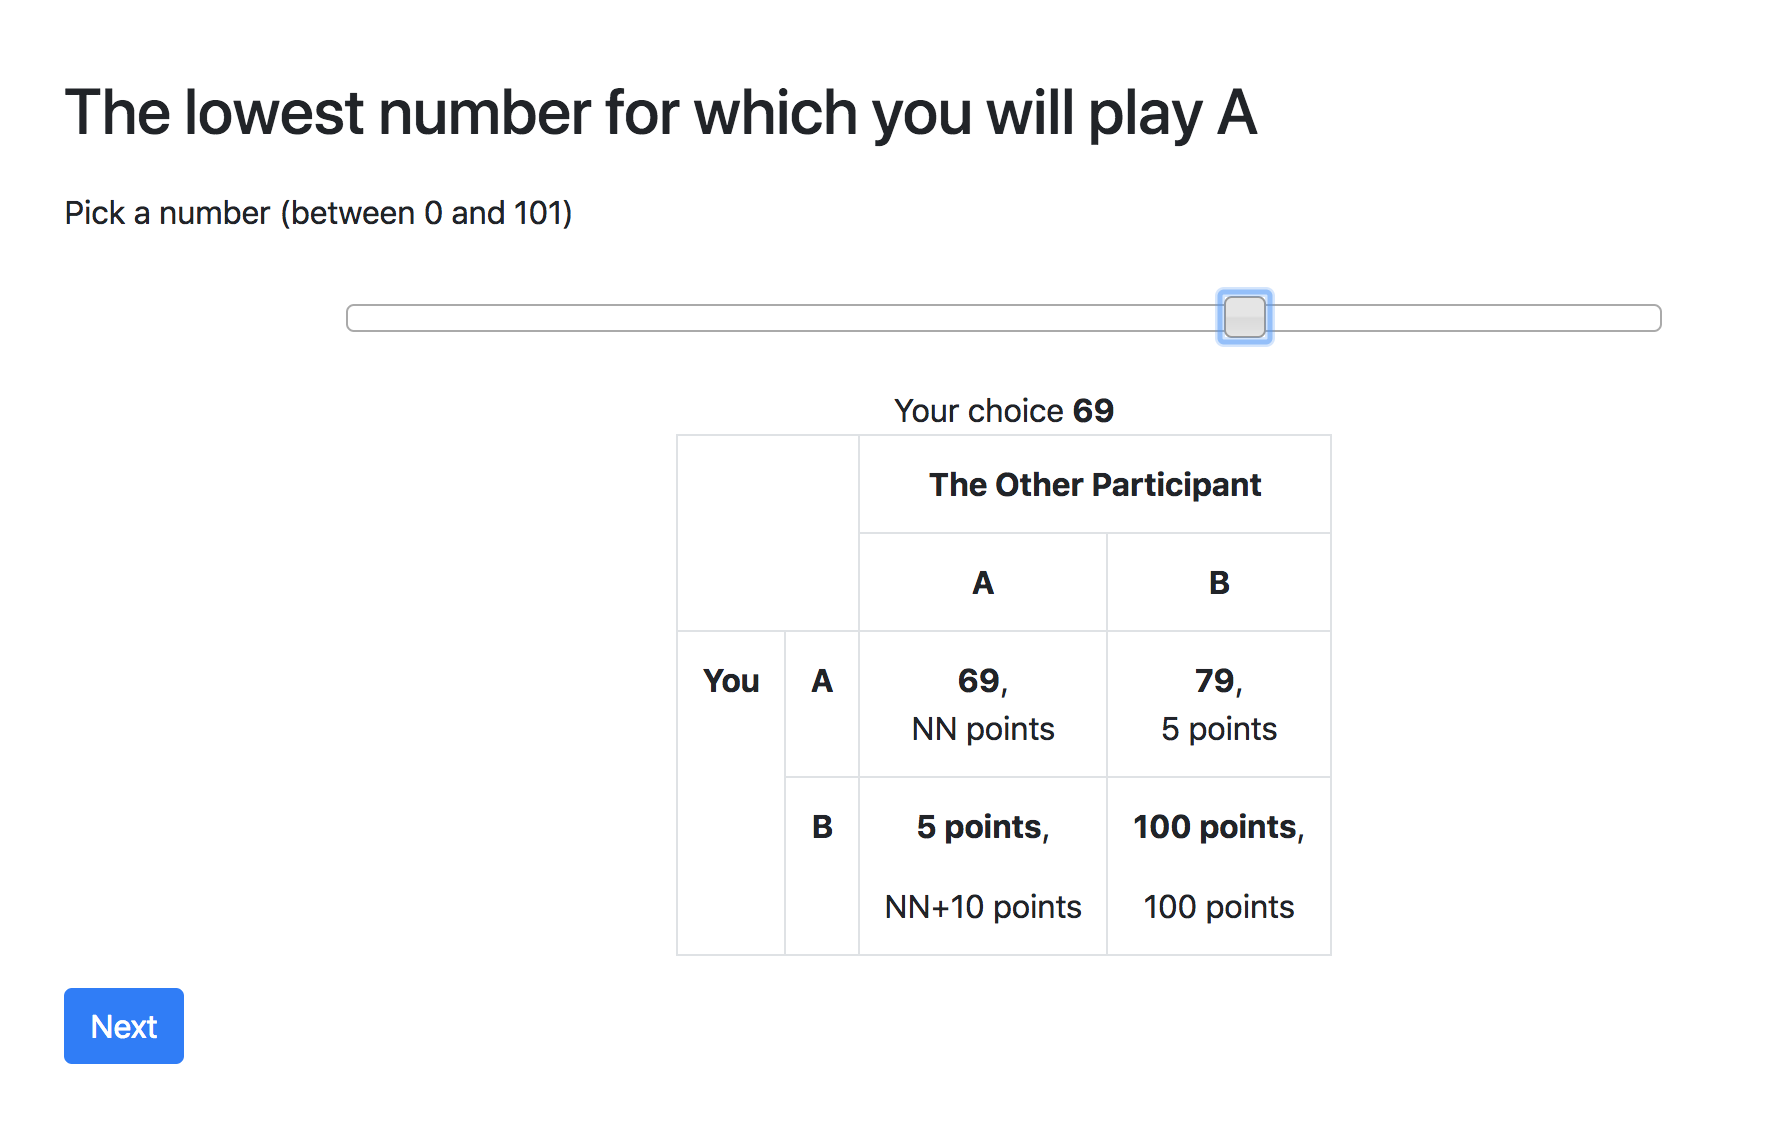
\includegraphics[scale=0.3]{cutoffen.png}%
\caption{User-Interface cutoff decision} 
\label{fig:ui}
\end{figure}
\end{center}





\begin{table}[ht]
\begin{center}

\caption{Timeline for each treatment}
\label{table:time}

\begin{tabular}{l|m{2.8cm}|m{3.5cm}|m{5cm}}
  Step & CGO & CGS & CGE\\
  \hline 
I & Cutoff & Cutoff & Cutoff \\
\hline
II& $x_i$ is revealed; D if $x_i< \text{cutoff}$ & $x_i$ is revealed; D if $x_i< \text{cutoff}$ for 1st mover (randomly chosen)
& $x_i$ is revealed; choose $t=\{1,2\}$ with action commitment defined according to \textit{cutoff}\\
\hline
III & - & 2nd mover picks \textbf{s} & 2nd mover ($t=2$) picks \textbf{s} if other chose $t=1$. Otherwise, the game is simultaneous.\\
\hline

\end{tabular}
\end{center}
\end{table}

In the CGO game, the value $x_i$ is revealed to subject $i$ and if the cutoff selected is smaller than or equal to revealed $x_i$, then the subject will play $H$, and $D$ otherwise. Following the actions, $H$ or $D$, of both subjects, payoffs are computed according to the payoff matrix in Table \ref{table:payoff}. In the CGS game, the first mover is randomly selected after all subjects select the cutoff point. This ensures that the cutoff decisions are independent of the imposed order of play, and allows us to have a fairly balanced number of silos across treatments. It is also important to emphasize that the subjects know that the cutoff decisions are binding (relaxed) for first (second) movers. The second mover picks an action $s\in\{H,D\}$ conditional on the first mover's action. That is, the second mover does not face the same payoff matrix as presented to the first mover. Instead, the payoff matrix in the CGS game for the second mover reflects the action selected by the first mover, and is thus reduced to a matrix with dimensions $2 \times 1$. In the CGE game, after $x_i$ is revealed, subjects choose the order of play. If both players select the same period of play, then the game becomes simultaneous. If one player picks the first period while the other player picks the second period, then the game is sequential and the cutoff choice for the second mover is relaxed. The second mover makes a decision knowing the action of the first mover. 

At the end of each round, for all treatments, we provide feedback regarding own and counterparty choices, as well as individual payoff information. Following 11 rounds of play, accumulated points over all rounds were converted to COP at the exchange rate of COP 20 per point. Earnings, including a show-up fee of COP 10,000 (USD 3.3), were paid in cash. On average, players earned 792.8 points (USD 5.2) for a session that lasted approximately 45 minutes. Table \ref{session} presents the average profit as well as other relevant information per treatment.\footnote{To provide context for our payments, the monthly minimum wage in Colombia was COP 781,281 when we ran the experiment. Assuming 20 workdays a month, and 8 hour workdays, we obtain an hourly rate of COP 4,483. Thus, the show-up fee of COP 10,000 is high enough to attract and incentivize people to participate in the experiment. On average, the participants earned a profit that was 1.5 times the show-up fee for an experiment which lasted less than one hour.} 
\begin{table}[ht]
\centering
\caption{Sessions overview }
\hline
\begin{tabular}{lcccc}
  Treatment & Silos & Subjects per silo & \% of women & Profit (mean, points)\\
  \hline  
  CGO & 6 & 12 & 51 & 701.6 \\
  CGS & 6 & 12 & 51 & 856.3 \\
  CGE & 6 & 12 & 47 & 820.7 \\
\hline
Total & 18 & 216 &  50 (mean) & 792.8 (mean)\\
\end{tabular}

\label{session}
\end{table}

\section{Results}
\label{sec:results}

We begin our analysis by presenting the average cutoff per period in the left panel of Figure \ref{fig:allcutoff}, which suggests learning across periods. While we observe a slight downward trend in the CGO treatment, the mean cutoff increases in the CGS and CGE treatments. The average cutoff does not reflect the heterogeneity of choices shown by the CDFs across treatments (right panel of Figure \ref{fig:allcutoff}). The CDF is constructed using the median cutoff choice by subject in rounds 6 through 11 to account for learning. We also present the NE predictions for the CGO and the CGS treatments as vertical lines. Recall that in the CGE game, equilibrium behavior can be consistent with either the CGO or the CGS game. \\

\noindent \textbf{Result 1}
\textit{The median cutoff strategy in the CGO game is 50.}\\

 In the CGO game, the median cutoff value is around 50, and the distribution of cutoffs is fairly uniform, with some qualifications. About 20\% of subjects pick the highest cutoff, which indicates that they strongly prefer to play $D$. Furthermore, we observe no significant mass centered around 33 as predicted in Hypothesis 1. In fact, the one-sample Wilcoxon test strongly rejects the hypothesis that the cutoff strategy in the CGO game is equal to the NE prediction (p-value $< 0.01$). Table \ref{tab(cutoffs)} shows the main cutoff statistics for all treatments, for all periods and for periods 6 through 11. \\
 
\begin{center}
\begin{figure}[ht]
\centering{}%
\begin{minipage}[t]{0.45\columnwidth}%
\subfloat{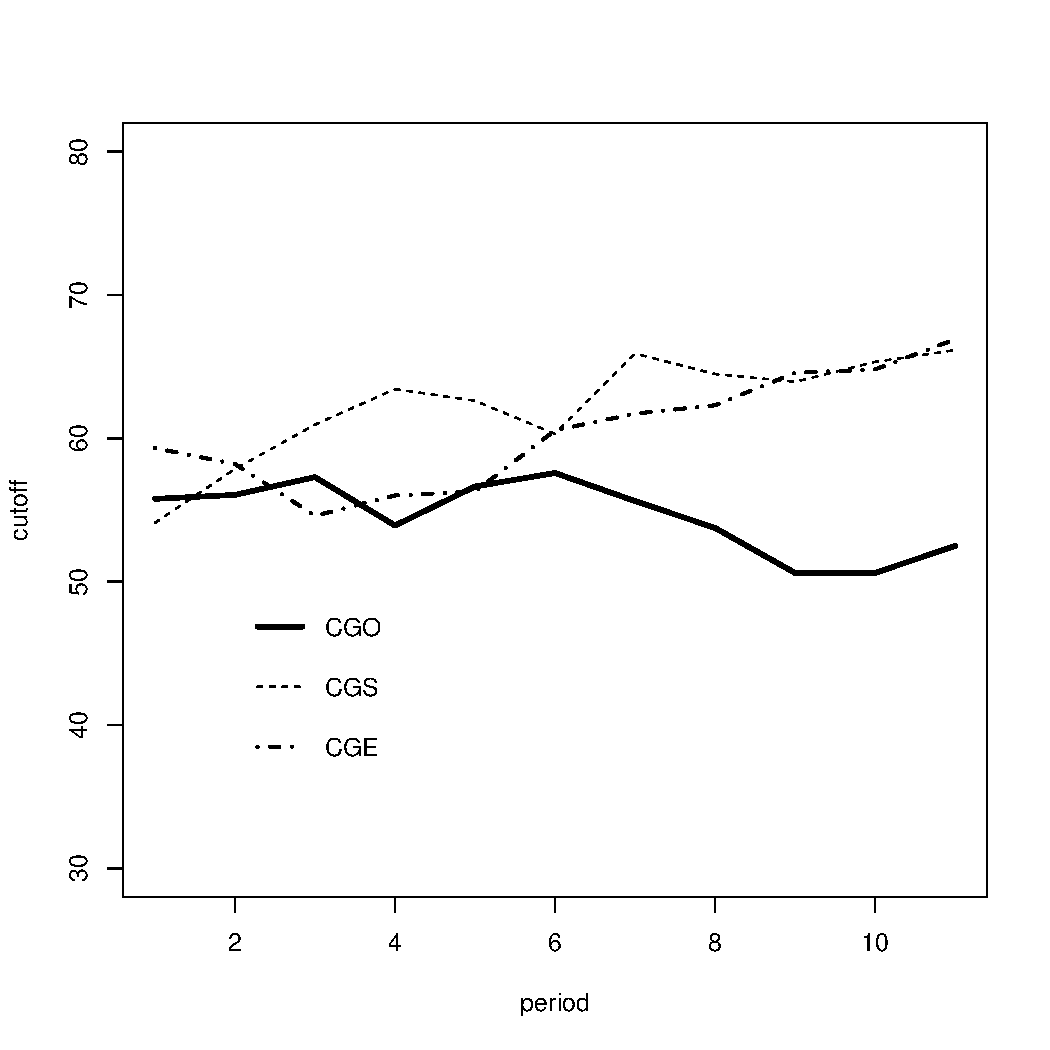
\includegraphics[scale=0.4]{periodcutoff.pdf}}%
\end{minipage}%
\begin{minipage}[t]{0.45\columnwidth}%
\subfloat{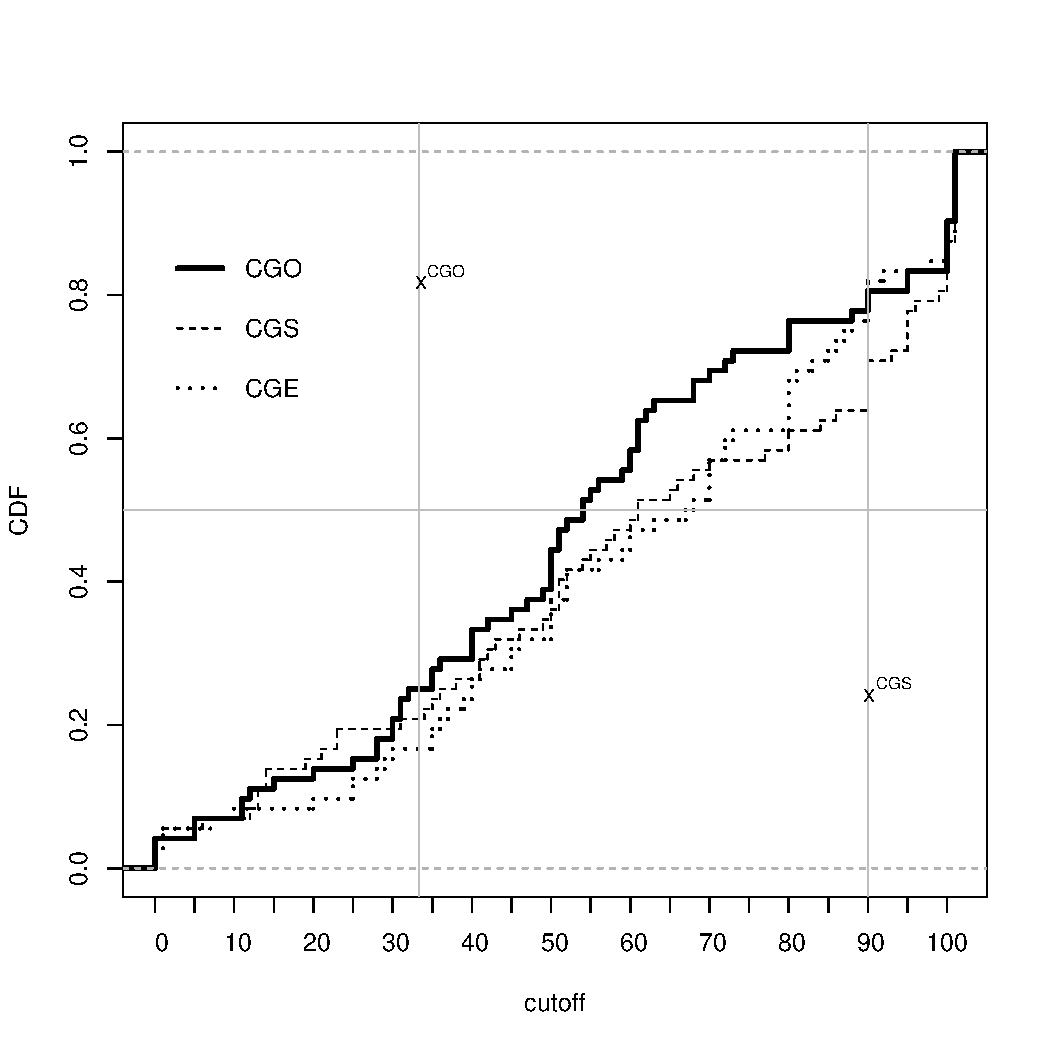
\includegraphics[scale=0.4]{cdfcutoff.pdf}}%
\end{minipage} 
%\captionsetup{font=large}
\caption{Mean cutoff per period (left) and CDF of subjects' cutoff strategies (right) \\\footnotesize{\textit{Note: $x^{CGO}$ ($x^{CGS}$) is the predicted cutoff in the CGO (CGS) game.}} }
\label{fig:allcutoff}\end{figure}
\par\end{center}

\begin{table}[!ht]
\centering\caption{Cutoffs by treatment (subject data)}

\begin{tabular}{lccc|ccc}
\hline
& \multicolumn{3}{c}{\textit{All Periods (1-11)}} & \multicolumn{3}{c}{\textit{Late Periods (6-11)}}\\
 & CGO & CGS  & CGE  & CGO & CGS  & CGE\\
  \hline
  NE prediction & 33 & 90 & \{33,90\} & 33 & 90 & \{33,90\}\\
  Mean & 56.10 & 61.93 & 62.07 &  53.17 &  64.38 & 64.03 \\
  SD & 30.30 & 33.18 & 29.04 &  31.90 &  31.90 & 29.47 \\
  Median & 54.00 & 61.00 & 67.50 &  50.00 &  65.75 & 69.50 \\
    N & 72 &  72 & 72 & 72 &  72 & 72 \\
\hline
\end{tabular}

\label{tab(cutoffs)}
\end{table}
\begin{table}[ht]
\centering\caption{ Wilcoxon test for cutoffs (p-values)}

\begin{tabular}{l|cc}
& CGS & CGE \\
\hline
CGE & = (0.789)& \\
CGO & $<$ (0.036) & $<$ (0.043)\\
\hline
 \multicolumn{3}{p{.35\textwidth}}{\scriptsize{Note: Each observation is the median cutoff of a subject in periods 6-11.}}\\ 
\end{tabular}

\label{tab(cutoff-pvalue)}
\end{table}
\\
\\
\noindent \textbf{Result 2}
\textit{In the CGS game, players increase the median cutoff to 66.}\\

The CDF for the CGS game in Figure \ref{fig:allcutoff} first-order stochastically dominates the CDF for the CGO game which confirms our Hypothesis 2 (p-value of a Wilcoxon test is 0.036, as shown in Table \ref{tab(cutoff-pvalue)}).\footnote{If we take an extremely conservative approach and work at the silo level, then the p-value is 0.093.} The mass in the CGS game moves toward the predicted NE of 90, though it still falls short. The median cutoff strategy is 66, and is different than the NE prediction (p-value $< 0.001$).  Similar to the CGO game, some players in the CGS game select either extremely high or extremely low cutoff values. Overall, the majority of players in the CGS game select a higher threshold relative to the players in the CGO game.\footnote{If we include all periods, then using a Wilcoxon test, we fail to reject that the CGO and the CGS distributions are equal. Significance of results (at 5\%) appears from periods 3 to 11.}\\


\noindent \textbf{Result 3}
\textit{In the CGE game, the median cutoff strategy is 70.}\\

The CDF for the CGE game in Figure \ref{fig:allcutoff} first-order stochastically dominates the CDF for CGO game (the p-value of a Wilcoxon test is 0.043 as shown in Table \ref{tab(cutoff-pvalue)}).\footnote{If we take an extremely conservative approach and work at the silo level, then we do not find a statistically significant difference across treatments.} When comparing subject choices across the CGE and CGS games, we fail to reject the hypothesis that the two cutoff choices come from the same distribution (see Table \ref{tab(cutoff-pvalue)}). The CDF for the CGE game shows that while roughly 25\% of players select a low cutoff strategy,  similar to the one in the CGO game (right panel of Figure \ref{fig:allcutoff}), the median cutoff is such that $\hat{x}_{_{CGE}}> \hat{x}_{_{CGO}}$. There is also a sizable mass (35\%) of players who select a cutoff strategy with values above the predicted NE of 90.


\begin{table}[ht]
\centering
\caption{Panel Regressions (cutoff)}
\footnotesize
\begin{tabular}{lccc}

  & (I) & (II) & (III) \\
&  cutoff & cutoff & cutoff   \\
&  (all periods) & (all periods)  & (all periods)   \\
    \hline
Intercept & $54.58^{^{***}}$ & $57.83^{^{***}}$ &  $ 57.53^{^{***}}$ \\
& (4.79) & (5.48) & (5.83) \\
CGS &  7.71 & $-1.24$ &  $-4.22$  \\
& (5.59) & (6.29) & (6.72) \\
CGE &  5.59 & $-3.47$ &  $-12.57^{^{*}}$ \\
& ( 5.54) &  (6.11) & (6.64) \\
Period & ---& $-0.54^{^{***}}$ & $-0.54^{^{***}}$ \\
& & (0.17)&  (0.17) \\
Period $\times$ CGS & ---& $1.49^{^{***}}$& $ 1.49^{^{***}}$ \\
& & (0.52) & (0.49)  \\
Period $\times$ CGE & ---& $1.56^{^{***}}$& $1.56^{^{***}}$\\
& & (0.36) & (0.35) \\
Men & --- &  --- & $0.61$  \\
& &  & (3.99) \\
Men $\times$ CGS & ---& --- &  6.13 \\
& & & (8.59) \\
Men $\times$ CGE & ---& --- & $17.20^{^{**}}$ \\
& & & (6.06)\\

\hline
N & 2,376 & 2,376 & 2,376 \\ 
$R^2$ & 0.01 & 0.02 & 0.04 \\
\hline
\hline
 \multicolumn{4}{p{.6\textwidth}}{\scriptsize{The dependent variable in (I)-(III)  is the cutoff choice. Standard errors are in parentheses, clustered at the group level and are computed via bootstrapping. Random effects are included at the subject level.}}\\ 
 \multicolumn{4}{p{0.4\textwidth}}{\scriptsize{ $^{^{***}}p\leq0.01$,
    $^{^{**}}p\leq0.05$, $^{^{*}}p\leq0.1$}} \\
\end{tabular}
\label{table:ols_cutoff}
\end{table}

To control for group effects we also perform panel regressions, presented in Table \ref{table:ols_cutoff}, which confirm our conclusions from the nonparametric analysis. In specification (I), we use all eleven periods, and cluster standard errors at the silo level and random effects at the subject level. In all, we evaluate three alternative specifications for cutoff choices using different regressors, including: $CGS$, which takes on the value of one when the treatment is a CGS game and zero otherwise, and $CGE$, which takes on the value of one when the treatment is a CGE game and zero otherwise. In Specifications (II-III), we include a trend variable $Period$, which controls for learning throughout the session, an interaction between the trend and the treatments, $Period \times CGS$ or $Period \times CGE$. We further include a gender variable $Men$, which takes on the value of one when the subject is a man and zero otherwise, and the interaction between gender and treatments, $Men \times CGS$ or $Men \times CGE$. We first focus on specifications (I-II) of Table \ref{table:ols_cutoff} and discuss the gender differences in Result 5. 

The mean cutoff choice in the CGO treatment (specification I) is about 54 which is above the NE prediction of 33. We do not find statistical differences across treatments without controlling for learning, as observed in specification (II), though the sign of the coefficient is consistent with the direction of the predictions. According to our predictions, the cutoff for CGS should be higher than in CGO. We find that the cutoff choice in the CGS treatment increases by about nine points over time.\footnote{The variable $Period$ is analyzed at the mean of six, when it is statistically significant.} This is also confirmed when we run a regression using the split sample 6-11 periods (see specification I of Table \ref{table:ols_cutoff_appendix} in Appendix C). In specification (II), we also find stronger significance using the trend variable which separates the negative trend behavior observed in the CGO game from the positive trend in the CGE game. Limiting the sample to periods 6-11, we find that treatment difference across CGE and CGO is significant at 10\% (see specification II of Table \ref{table:ols_cutoff_appendix} in Appendix C) which suggest higher heterogeneity across choices in the CGE treatment due to the multiplicity of equilibria. 

Next, we analyze the joint distribution of outcomes in all treatments by counting the frequency of each outcome ($HH$, $HD$, $DH$ and $DD$) for each treatment (see Table \ref{tab(cells)}). Recall that in the CGO game the average cutoff (about 54) is above the NE prediction (of 33). This means that we are less likely to observe the $HH$ outcome compared to the NE prediction. For example, given a cutoff of 54, the expected probability of $HH$ play is  about 22\%\footnote{Given a cutoff value of $y$, the probability of playing $H$ is $(101-y)/101$.} which is not that far from the empirical frequency of 19\% reported in Table \ref{tab(cells)}. Likewise, the expected probability of $DD$ is 29\%, close to the empirical frequency of 31\% reported in Table \ref{tab(cells)}. We reject that outcome  $HH$ and $DD$ are equal to the NE prediction (p-value $< 0.001$) respectively.\footnote{The cell outcome is tested by running an OLS regression using joint choices, and performing a Wald-test for the coefficient restrictions.} In the CGS game, where the cutoff is binding for the first mover (selected via a fair coin flip) only and the observed mean cutoff is 62, the expected probability of $H$ for the first mover is 39\%. For the second mover, the expected probability of not being a dominant strategy dove is 95\%. Thus, assuming that second mover is best responding, the probability of $HH$ in the CGS game is 37\%, which follows closely the empirical distribution of 39.39\% reported in Table \ref{tab(cells)}. The NE predicts a smaller probability for $HH$ play given the cutoff prediction of 90. The data shows that, conditional on the first mover playing $H$, 90\% of the observations are consistent with a best response strategy.

\begin{table}[ht]
\centering\caption{Frequency (\%) of outcomes}
\footnotesize
\begin{tabular}{lcc|cc|ccc}
\hline
Outcome & \multicolumn{2}{c|}{CGO} & \multicolumn{2}{c|}{CGS} & \multicolumn{3}{c}{CGE -- Data}\\
 & NE & Data & NE & Data & One-shot 1st period & One-shot 2nd Period & Sequential\\
  &  &  &  &  & (\% of 1st period) & (\% of 2nd period) & (\% of Sequential)\\
 \hline
$HH$ & 44.89 & 18.94 & 9.50& 39.39& 2.27  & 5.56& 17.93 \\
 &  &  & & &(16.97) & (16.19) & (34.30) \\
  $HD$ &22.11 & 24.88 & 0.50 & 5.81 & 2.90 & 7.95 & 3.29 \\
  && &  & & (21.67)&  (23.14) &  (6.29)\\
  $DH$ &22.11 & 24.88& 9.00 & 6.06 & 2.90  &7.95 & 1.76 \\
    && & &  &(21.67) & (23.14) &  (3.37)\\
  $DD$ & 10.89 & 31.31& 81.00 &48.74 & 5.30  & 12.88 & 29.29 \\
    &  & &  & & (39.61) &  (37.50)&  (57.20)\\
Total & 100 &100 &100 &100 & 13.38 & 34.35 & 52.27\\
 &  & & & &  (100)&  (100) & (100)\\
\hline   
\multicolumn{8}{p{1\textwidth}}{\scriptsize{Note: $HD$ denotes that the first player (mover) plays $H$ while the second player (mover) plays $D$. For the one-shot game we count as a single cell $HD$ or $DH$ and present the equal split for $HD$ and $DH$. Due to rounding, the numbers may not necessarily add up to 100. The number in parenthesis for CGE game represents the frequency of cells observed within an encounter type.}}\\ 
\end{tabular}
\label{tab(cells)}
\end{table}

The higher frequency of $HH$ play in the CGS game translates into a lower frequency of $DD$ play (48\%) relative to the NE prediction. One would expect that, conditional on the probability of first mover playing $D$ with 61\%, the second mover will also play $D$ if she is not a hawk dominant type (10\%). Thus, the expected probability of observing $DD$ would be 55\%, which is close to the observed frequency of 48.74\% reported in Table \ref{tab(cells)}. Overall, we find that conditional on the first mover playing $D$, 98\% of the observations are consistent with a best response strategy. Thus, the outcome $DH$ reflects the hawk dominant who best respond to $D$. We reject that the outcomes $HH$ and $DD$ in the CGS game are equal to the NE prediction (p-value $<0.001$). When comparing the outcomes $HH$ and $DD$ across CGS and CGO, we find that the frequency of $HH$ is weakly higher in the CGS game (p-value $=0.09$) while the frequency of $DD$ is significantly higher (p-value $=0.04$). 

The CGE game outcome can resemble either that of a CGO game or a CGS game. Overall, $HH$ appears in about 25\% (=2.27\%+5.56\%+17.93\%) of the observations, which is between the values observed in CGO and CGS games. The outcome $DD$ appears in about 47\% of the observations which is closer to the $DD$ outcome in the CGS game. The off-diagonals cells are therefore higher than in the CGS game but lower than what we observe in the CGO game. We do not find a statistically significant difference in the $HH$ outcomes across CGO and CGE games (p-value $=0.91$), while for the $DD$ outcome the frequency is higher in the CGE game relative to the CGO game (p-value $=0.04$). \\

\noindent \textbf{Result 4} \textit{Social welfare is higher in the CGS and CGE environments.}\\

The analysis of joint outcomes in Table \ref{tab(cells)} shows that coordination of $HH$ and $DD$ play in the CGS game is higher than in the CGO game, which leads to large social welfare gains. While $DD$ offers higher welfare gains, since joint profit can reach a maximum of 200, $HH$ also leads to higher welfare compared to the off-diagonal cells when $x>15$.\footnote{For example, consider that one player with type $y$ plays $H$, and other player of type $x$ plays $D$. In the CGO game, the social welfare is $y+10+5$ while in the CGS game, assuming that both players play $H$, the social welfare is $y+x$. Thus, the social welfare for playing $HH$ is higher than playing $HD$ if $x>15$.} We formally test the difference of social welfare across treatments in Table \ref{table:ols_jointprofit}. In specification (I), which includes all periods, we find that social welfare is higher by 20 points in the CGS game and about 15 points in the CGE game, compared to the CGO game. When we restrict the sample to late periods (6-11), the results remain the same (see specification III of Table \ref{table:ols_cutoff_appendix} in Appendix C). Alternatively, we include a trend variable (Period) in Specification (II) with treatment interactions. While we find that $Period$ is not significant for the CGO and CGS games, in the CGE game there is an increase of joint profit over time.\\

\begin{table}[ht]
\centering
\caption{Panel regressions (social welfare)}
\footnotesize
\begin{tabular}{lcc}
\hline
  & (I) & (II)  \\
&  joint profit   & joint profit  \\
&  (all periods)   & (all periods) \\
    \hline
Intercept & $95.96^{^{***}}$  &$ 96.01^{^{***}}$ \\
& (4.12) & (8.59)  \\
CGS &  $20.24^{^{***}}$  & $ 19.70^{^{**}}$ \\
& (4.79)  & (10.00)  \\
CGE &  $15.47^{^{**}}$ & $-3.47$  \\
& (6.44)   & (5.77)  \\
Period & ---&$-0.00$ \\
&  & (0.76)\\
Period $\times$ CGS & ---&$0.09$ \\
&  & (0.91)   \\
Period $\times$ CGE & ---&$1.63^{^{**}}$\\
&  & (0.82)  \\

\hline
N & 1,188  & 1,188 \\ 
$R^2$ & 0.02  & 0.02  \\
\hline
\hline
 \multicolumn{3}{p{.7\textwidth}}{\scriptsize{The dependent variable in (I)-(II) is the sum of profit across pairs. Standard errors are in parentheses, clustered at the silo level and are computed via bootstrapping.}}\\ 
 \multicolumn{3}{p{0.4\textwidth}}{\scriptsize{ $^{^{***}}p\leq0.01$,
    $^{^{**}}p\leq0.05$, $^{^{*}}p\leq0.1$}} \\
\end{tabular}
\label{table:ols_jointprofit}
\end{table}

\noindent \textbf{Result 5}
\textit{Gender differences appear only in the CGE game. Men significantly increase their cutoff choices, improving the frequency with which $D$ is selected, while women revert to a strategy similar to the one in the CGO game. The men who commit to $D$ move first more often than those who commit to $H$.}\\

The CGE game shows a similar frequency of $DD$ outcome as the CGS game. The mean cutoff by gender, however, is quite different. The cutoff strategy chosen by women in the CGE game is similar to their cutoff strategy in the CGO game. The men, on the other hand, increase their cutoff strategies, relative to the CGO game. Figure \ref{fig:cdfgender1} presents the CDF of cutoff strategies by gender in the CGO game (left panel) and the CGS  game (right panel). We fail to reject that the cutoffs are equal across gender in both CGO and CGS treatments. Furthermore, in the CGS game, conditional on observing $D$ in the first period, we do not observe any gender differences in the response of the second mover. 
\begin{center}
\begin{figure}[ht]
\centering{}%
\begin{minipage}[t]{0.45\columnwidth}%
\subfloat{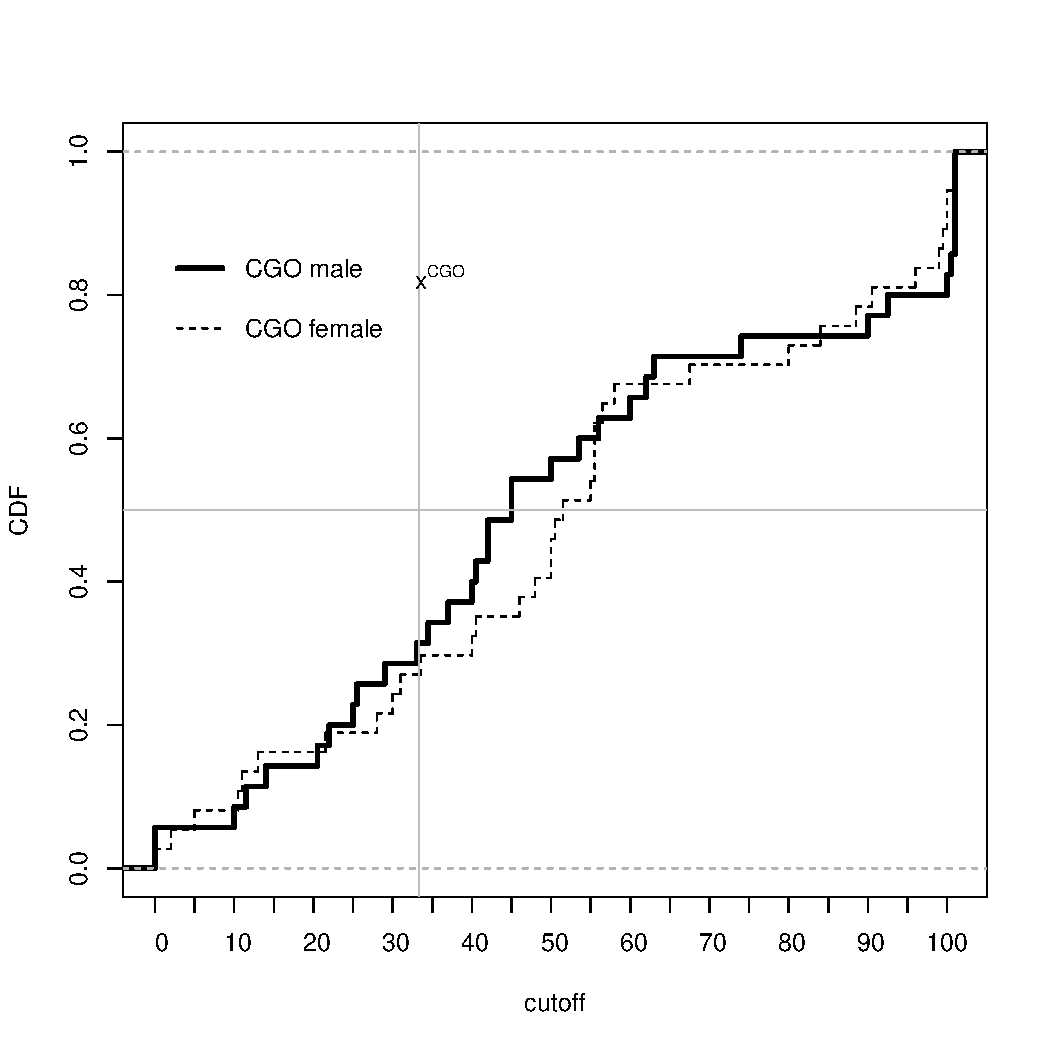
\includegraphics[scale=0.4]{cdfcutoffgender_o.pdf}}%
\end{minipage}%
\begin{minipage}[t]{0.45\columnwidth}%
\subfloat{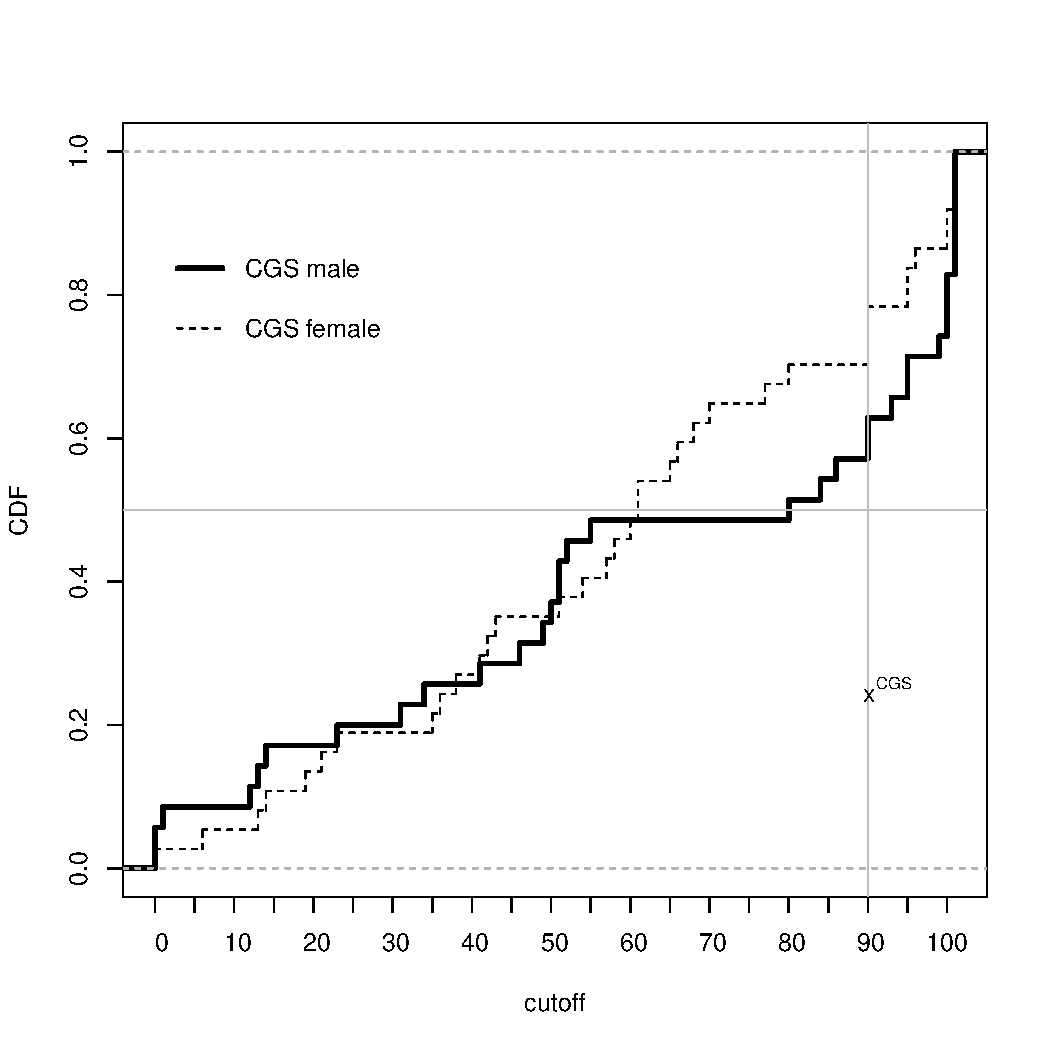
\includegraphics[scale=0.4]{cdfcutoffgender_s.pdf}}%
\end{minipage} 
%\captionsetup{font=large}
\caption{CDF of cutoff strategy choices in CGO (left) and CGS (right), by gender \\\footnotesize{\textit{Note: $x^{CGO}$ ($x^{CGS}$) is the predicted cutoff in the CGO (CGS) game.}} }
\label{fig:cdfgender1}\end{figure}
\par\end{center}

The cutoff strategy choices in the CGE game by men first order stochastically dominate the cutoff strategy choices by women, which we depict in the left panel of Figure \ref{fig:cdfgender2}. We reject the null hypothesis which states that men choose a cutoff strategy that is equal to the one chosen by women (p-value $<0.001$). The higher cutoff choices by men lead to higher frequency of $D$.\footnote{Using all periods, we also confirm the separation between cutoffs (p-value of 0.06). The difference in $D$ play across gender is significant at a 5\% significance level in the regression analysis, see Table \ref{table:ols_all} in Appendix C.} Table \ref{table:ols_cutoff} also presents gender differences using panel (OLS) regressions. According to specification (III), the variable $Men$ is only significant in the CGE treatment. Women use a cutoff similar to the one in the CGO treatment ($1.56\times 6-12.57= -3.21$) while men increase their cutoffs relative to women by 17 points in the CGE treatment. The gender difference in the CGE game is robust when we focus on periods 6-11 of the sample (see specification II of Table \ref{table:ols_cutoff_appendix} in Appendix C). Therefore, our results show that different motivations of play across gender can be manifested in an endogenous timing game. The fear of being exploited triggers a cutoff similar to the CGO game for women, while men, who are motivated by profit, select a cutoff similar to the one in the CGS game. 

\begin{center}
\begin{figure}[ht]
\centering{}%
\begin{minipage}[t]{0.45\columnwidth}%
\subfloat{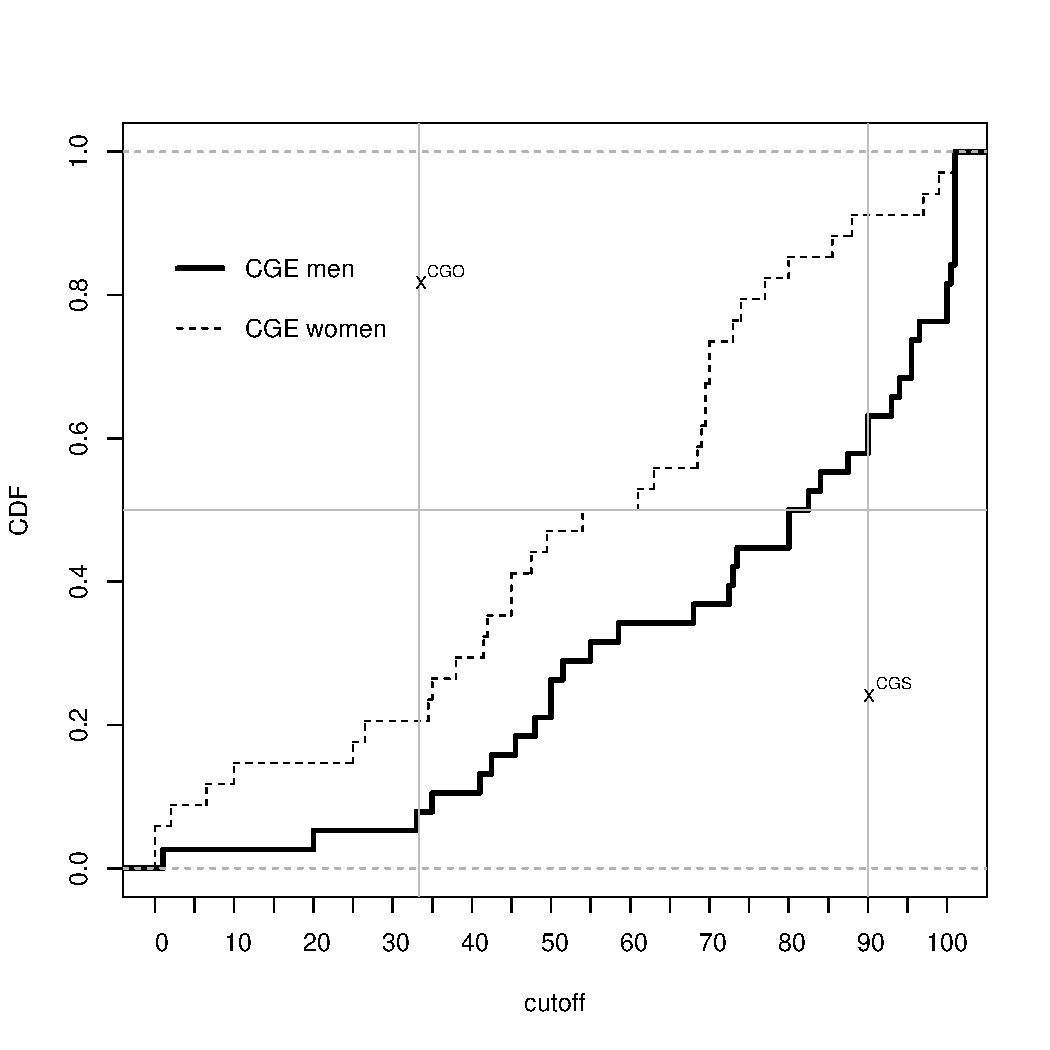
\includegraphics[scale=0.4]{cdfcutoffgender_e1.pdf}}%
\end{minipage}%
\begin{minipage}[t]{0.45\columnwidth}%
\subfloat{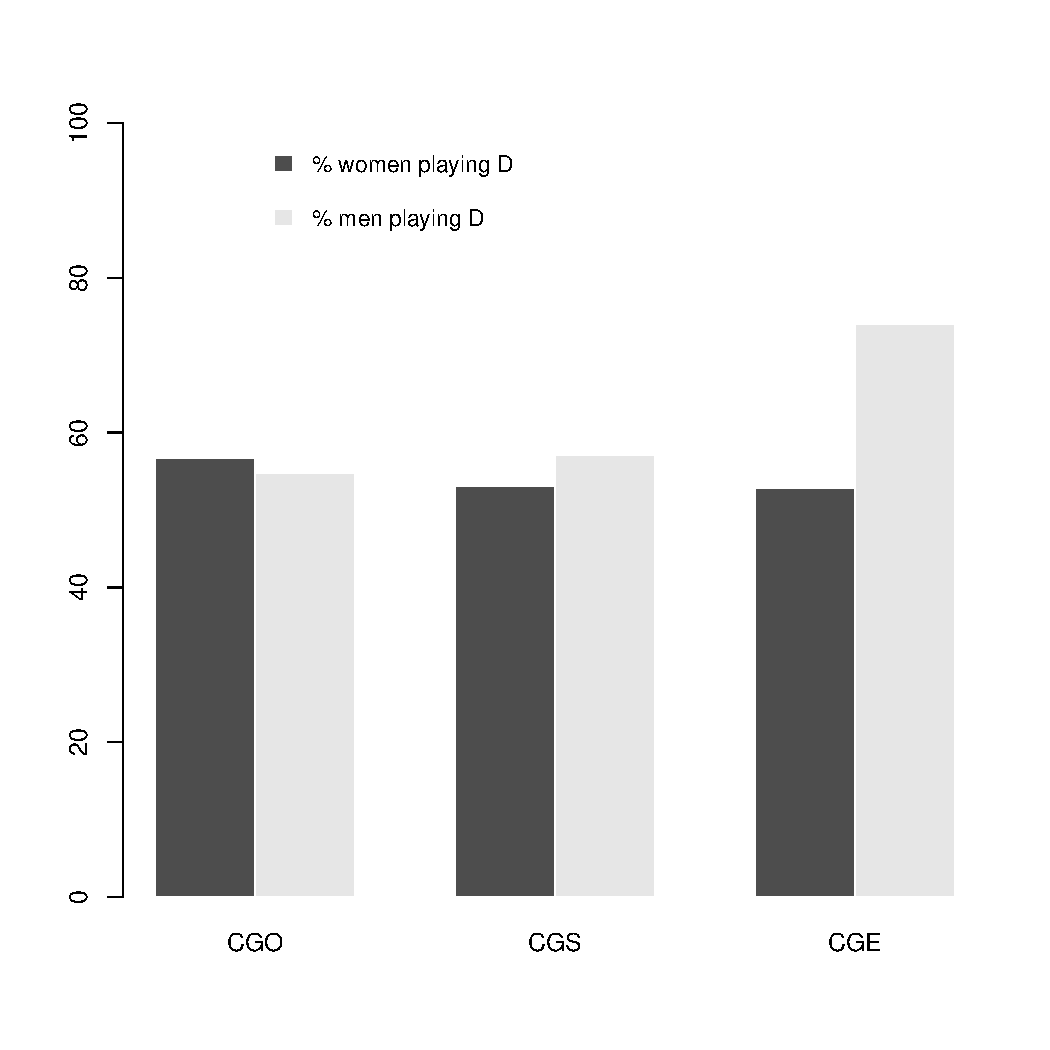
\includegraphics[scale=0.4]{genderplay1.pdf}}%
\end{minipage} 
%\captionsetup{font=large}
\caption{CDF of cutoff strategies in CGE (left panel) and $D$ play (right panel) by gender\\ \footnotesize{\textit{Note: $x^{CGO}$ ($x^{CGS}$) is the predicted cutoff in the CGO (CGS) game.}}}
\label{fig:cdfgender2}\end{figure}
\par\end{center}

Next, we analyze gender differences in the CGE game based on the order of play. We run a logit regression in Table \ref{table:move_cge} which includes individual random effects and clustered standard errors by silo (12 subjects). The dependent variable is the timing of play (which takes the value of one when a player moves second, and zero otherwise), while the independent variable \textit{D commitment}, in specification (I), is a binary variable that takes the value of one when the player commits to $D$, and zero otherwise. Recall that after a player selects a cutoff, the value of $x$ is revealed, and the player then decides whether to move first or second. \textit{D commitment} captures the decision to play $D$ if the game is a simultaneous move game, or the player is the first mover. According to specification (I), the likelihood of choosing to move second is higher than choosing to move first. The commitment to $D$ is not significant but the negative sign on the coefficient follows the predicted direction of the CGS equilibrium, which implies that a first mover has strong incentive to set the stage by playing $D$. 

In specification (II) of Table \ref{table:move_cge}, we include the gender variable $Men$ as well as an interaction term. The significance of the negative coefficient on the interaction term shows that men who commit to $D$ move first more frequently than those who commit to $H$, which is consistent with the CGS equilibrium. The (log) odds that a man who commits to $H$ will move second increases by 1.26, while a man who commits to $D$ is less likely to move second (a decrease in the log-odds of  $-0.72$). We do not find statistical differences in the odds for women. That is, they randomly select to move across both periods. This behavior is consistent with the cutoff choice in the simultaneous game. A player who believes that the game is simultaneous is indifferent between the first and second period of play. The results are robust when we control for Period in specification (III) of Table \ref{table:move_cge}, which captures learning effects. 

\begin{table}[ht]
\centering
\caption{Panel Regressions (logit)}
\footnotesize
\begin{tabular}{lcccc}

  & (I) & (II) & (III) \\
&  Move 2nd period &  Move 2nd period & Move 2nd period\\
    \hline
Intercept &  $.71^{^{***}}$ & .11 & .48\\
& ( .25) & (.42) & (.37) \\
D commitment & $-.08$ & .22& .24\\
& (.30) & (.38) & (.36) \\
Men & -- &  $1.26^{^{**}}$ &  $1.24^{^{**}}$\\
& & ( .54) & (.53) \\
D commitment $\times$ Men & -- & $-.72^{^{**}}$ & $-.70^{^{**}}$\\
& & ( .28) & (.27) \\
Period & -- & --& $-.06^{^{*}}$\\
& & & (.03) \\

\hline
N & 792 & 792 & 792 \\ 
$\chi^2$ &  0.08  &  7.78 &  16.74\\
\hline
\hline
 \multicolumn{4}{p{.8\textwidth}}{\scriptsize{Note: All specifications run a logit regression in which the dependent variable take the value of one when a player moves second. The regressors include (i) commitment to $D$, which takes the value of one when $D$ and zero otherwise, (ii) dummy for men, which takes the value of one when the subject is male, and zero otherwise, and (iii) trend $Period$. Standard errors are in parenthesis, clustered at the silo level and are computed via bootstrapping. Random effects are included at the subject level. }}\\ 
 \multicolumn{4}{p{0.4\textwidth}}{\scriptsize{ $^{^{***}}p\leq0.01$,
    $^{^{**}}p\leq0.05$, $^{^{*}}p\leq0.1$}} \\
\end{tabular}
\label{table:move_cge}
\end{table}


\section{Discussion}
\label{sec:discuss}

In this paper, we provide a theoretical model and experimental evidence on how strategic commitment can enhance social welfare in conflict scenarios. The experimental design includes: (i) a simultaneous game; (ii) a sequential order of play; and (iii) an endogenous order of play. We also study whether gender differences play a role in strategic behavior in conflict games of incomplete information. Our results show that a sequential order of play improves welfare relative to the simultaneous game. Gender is not important in explaining behavior of either the sequential or the simultaneous move game. However, when players are allowed to self-select the order of play, we find that women prefer to move first and adopt a cutoff similar to the one in the simultaneous-move game, while men adopt a cutoff similar to the one in the sequential game. We find that men who commit to $D$ are less likely to move second, which follows the prediction of a separating equilibrium. 

Our results provide important insights into a variety of games of incomplete information. First, the strategic interaction of players is similar across gender for some classes of games and therefore, one should not be surprised if gender differences are not always observed. This is consistent with previous literature which does not find strong evidence of gender differences in simultaneous move Prisoners Dilemma and Stag Hunt games. Second, there is a large heterogeneity in choices within each gender. Using a slider to elicit cutoffs, we are able to observe the values which trigger Hawkish play. Third, differences in motivations across gender become important in the endogenous timing game. Men prefer to wait and see the action of the first mover when they commit to $H$, and prefer to move first when they commit to $D$. Women, on the other hand, select a cutoff similar to the simultaneous move game, thus increasing the frequency of $H$ play. Our experimental design cannot explain the source of these different motivations. We hope that our findings motivate further research on the role of gender in conflict games in which actions are characterized as strategic complements, such as negotiations, and corporate disputes.


\section{Acknowledgments}
We are grateful for the comments received from the Editor Daniela Puzzello, three anonymous referees, Ann O'Leary Grossman, Lata Gangadharan, Marie Claire Villeval, Erte Xiao, Dan Friedman, Tomas Sj\"ostr\"om, Dann Arce, Nisvan Erkal, Diego Aycinena, Kyung Hwan Baik, Erik Kimbrough, Tim Cason, Tom Wilkening, Roman Sheremeta, Maria Recalde, John Duffy, Jin Yeub Kim, and seminar participants in numerous seminars and conferences. This research was supported by funds granted by Colby College. This project was approved by the IRB at Colby College and Universidad del Rosario.

\newpage
\begin{thebibliography}{10}

%\bibitem{} Andreoni, J., 1998. Toward a theory of charitable fund-raising. \textit{Journal of Political Economy,} 106(6), pp.1186-1213.

%\bibitem{} Avoyan, A., 2019. Communication in global games: theory and experiment. 

%\bibitem{} Azmat, G., Calsamiglia, C. and Iriberri, N., 2016. Gender differences in response to big stakes. \textit{Journal of the European Economic Association,} 14(6), pp.1372-1400.

\bibitem{} Babcock, L., Recalde, M.P., Vesterlund, L. and Weingart, L., 2017. Gender differences in accepting and receiving requests for tasks with low promotability. \textit{American Economic Review,} 107(3), pp.714-47.

%\bibitem{} Baik, K.H. and Shogren, J.F., 1992. Strategic behavior in contests: comment. \textit{The American Economic Review,} 82(1), pp.359-362.

\bibitem{key-32}  Baliga, S. and Sj\"ostr\"om, T., 2004. Arms Races and Negotiations. \textit{Review of Economic Studies} 71, pp. 351-369.

%\bibitem{} Baliga, S, and Sj\"ostr\"om, T. 2009. Conflict Games with Payoff Uncertainty. Unpublished.

%\bibitem{} Baliga, S, and Sj\"ostr\"om, T. 2012. The Hobbesian Trap. In \textit{The Oxford Handbook of the Economics of Peace and Conflict,} edited by Michelle R. Garfinkel and Stergios Skaperdas. New York: Oxford University Press.

%\bibitem{key-32}  Baliga, S. and Sj\"ostr\"om, T., 2012. The Strategy of Manipulating Conflict.\textit{American Economic Review} 102 (6), pp. 2897-2922.

%\bibitem{key-32} Benndorf, V., Martinez-Martinez, I. and Normann, H.T., 2016. Equilibrium selection with coupled populations in hawk-dove games: Theory and experiment in continuous time. \textit{Journal of Economic Theory,} 165, pp.472-486.

\bibitem{key-32} Brindisi, F., \c{C}elen, B. and Hyndman, K., 2014. The effect of endogenous timing on coordination under asymmetric information: An experimental study. \textit{Games and Economic Behavior,} 86, pp.264-281.

\bibitem{} Cabrales, A., Nagel, R. and Armenter, R., 2007. Equilibrium selection through incomplete information in coordination games: an experimental study. \textit{Experimental Economics,} 10(3), pp.221-234.

\bibitem{} Carlsson, H. and Van Damme, E., 1993. Global games and equilibrium selection. \textit{Econometrica: Journal of the Econometric Society,} 61(5) pp.989-1018.

%\bibitem{} Casari, M., Ham, J.C. and Kagel, J.H. 2007. Selection bias, demographic effects, and ability effects in common value auction experiments. \textit{American Economic Review,} 97, pp.1278-1304.

\bibitem{key-32} Chen, D.L., Schonger, M. and Wickens, C., 2016. oTree--An open-source platform for laboratory, online, and field experiments. \textit{Journal of Behavioral \& Experimental Finance,} 9, pp.88-97.

%\bibitem{key-32} Chen, Y., Katuscak, P. and Ozdenoren, E. 2013. Why can't a woman bid more like a man? \textit{Games and Economic Behavior,} 77, pp.181-213.

%\bibitem{key-32} Chen, Z., Ong, D. and Sheremeta, R. 2015. The Gender Difference in the Value of Winning, \textit{Economics Letters,} 137, pp.226-229.

%\bibitem{key-32} Crosetto, P. and Filippin, A., 2017. Safe options induce gender differences in risk attitudes.

%\bibitem{key-32} Dasgupta, A. 2007. Coordination and Delay in Global Games. \textit{Journal of Economic Theor,} 134(1), pp.195-225.

%\bibitem{key-32} Di Girolamo, A. and Drouvelis, M., 2015. The role of gender composition and size of the group in a minimum effort game. \textit{Economics Letters,} 137, pp.168-170.

\bibitem{key-32} Dijk, O., 2017. Bank run psychology. \textit{Journal of Economic Behavior \& Organization,} 144, pp.87-96.

%\bibitem{key-32} Duan, J., Kobayashi, H. and Shichijo, T., 2019. Does cheap talk promote coordination under asymmetric information? An experimental study on global games. An Experimental Study on Global Games, mimeo.

\bibitem{} Duffy, J. and Ochs, J., 2012. Equilibrium selection in static and dynamic entry games. \textit{Games and Economic Behavior,} 76(1), pp.97-116.

%\bibitem{} Dufwenberg, M. and Gneezy, U., 2005. Gender \& coordination.In \textit{Experimental business research} (pp. 253-262). Springer, Boston, MA.

%\bibitem{} Eaton, C.B., 2004. The elementary economics of social dilemmas. \textit{Canadian Journal of Economics/Revue canadienne d'\'{e}conomique,} 37(4), pp.805-829.

\bibitem{key-32}  Evdokimov, P. and Garfagnini, U., 2018. Third-party manipulation of conflict: an experiment. \textit{Experimental Economics,} 21(1), pp.27-49.

\bibitem{key-32}  Farrell, J. and Saloner, G., 1985. Standardization, compatibility, and innovation. \textit{the RAND Journal of Economics,} pp.70-83.

\bibitem{} Gangadharan, L., Jain, T., Maitra, P. and Vecci, J., 2019. Female leaders and their response to the social environment. \textit{Journal of Economic Behavior \& Organization,} 164, pp.256-272.

%\bibitem{key-32}  Gill, D. and Prowse, V., 2014. Gender differences and dynamics in competition: The role of luck. \textit{Quantitative Economics,} 5(2), pp.351-376.

%\bibitem{} Goldstein, I. and Pauzner, A., 2004. Contagion of self-fulfilling financial crises due to diversification of investment portfolios. \textit{Journal of Economic Theory,} 119(1), pp.151-183.

%\bibitem{} Goldstein, I. and Pauzner, A., 2005. Demand-deposit contracts and the probability of bank runs. \textit{Journal of Finance,} 60(3), pp.1293-1327.

\bibitem{} Greiner, B., 2015. Subject pool recruitment procedures: organizing experiments with ORSEE. \textit{Journal of the Economic Science Association,} 1(1), pp.114-125.

%\bibitem{} Grossman, P.J., Komai, M. and Jensen, J.E., 2015. Leadership and gender in groups: An experiment. \textit{Canadian Journal of Economics,} 48(1), pp.368-388.

%\bibitem{}  Guimaraes, B. and Morris, S., 2007. Risk and wealth in a model of self-fulfilling currency attacks. \textit{Journal of Monetary Economics,} 54(8), pp.2205-2230.

%\bibitem{}  Ham, J.C. and Kagel, J.H. 2006. Gender effects in private value auctions. \textit{Economic Letters,} 92, pp.375-382.

\bibitem{} Hamilton, J.H., and Slutsky, S.M. 1990. Endogenous Timing in Duopoly Games: Stackelberg or Cournot Equilibria. \textit{Games and Economic Behavior} 2, pp.29-46

\bibitem{} Heggedal, T.R., Helland, L. and Joslin, K.E.N., 2018. Should I Stay or should I Go? Bandwagons in the lab. \textit{Journal of Economic Behavior \& Organization,} 150, pp.86-97.

\bibitem{}Heinemann, F., Nagel, R. and Ockenfels, P., 2004. The theory of global games on test: experimental analysis of coordination games with public and private information. \textit{Econometrica, } 72(5), pp.1583-1599.

%\bibitem{} Heinemann, F., Nagel, R. and Ockenfels, P., 2009. Measuring strategic uncertainty in coordination games. \textit{The Review of Economic Studies,}  76, pp.181-221

%\bibitem{}Huck, S., M\"{u}ller, W. and Normann, H.T., 2001. Stackelberg beats Cournot-on collusion and efficiency in experimental markets. \textit{The Economic Journal,} 111(474), pp.749-765.

%\bibitem{}Huck, S., M\"{u}ller, W. and Normann, H.T., 2002. To commit or not to commit: endogenous timing in experimental duopoly markets. \textit{Games and Economic Behavior,} 38(2), pp.240-264.

\bibitem{} Ingram, B.L. and Berger, S.E., 1977. Sex-role orientation, defensiveness, and competitiveness in women. \textit{Journal of Conflict Resolution,} 21(3), pp.501-518.

%\bibitem{} Jetter, M. and Walker, J.K., 2018. The gender of opponents: Explaining gender differences in performance and risk-taking?. \textit{European Economic Review,} 109, pp.238-256.

\bibitem{} Khan, H., 2017. Essays in the experimental analysis of conflict. University of Birmingham. Ph.D.

\bibitem{} Kiss, H.J., Rodriguez-Lara, I. and Rosa-Garcia, A., 2014. Do women panic more than men? An experimental study of financial decisions. \textit{Journal of Behavioral and Experimental Economics,} 52, pp.40-51.


\bibitem{} Kimbrough, E.O., Laughren, K. and Sheremeta, R., 2017. War and conflict in economics: Theories, applications, and recent trends. \textit{Journal of Economic Behavior \& Organization}

\bibitem{} Kuwabara, K., 2005. Nothing to fear but fear itself: Fear of fear, fear of greed and gender effects in two-person asymmetric social dilemmas. \textit{Social Forces,} 84(2), pp.1257-1272.


%\bibitem{} Li, K.K., 2011. Preference towards control in risk taking: Control, no control, or randomize?. \textit{Journal of Risk and Uncertainty,} 43(1), pp.39-63.

%\bibitem{} Kop\'{a}nyi-Peuker, A.A., 2018. \textit{Yes, I'll do it: a large-scale experiment on the volunteer's dilemma} (No. 18-072/II). Tinbergen Institute.

%\bibitem{} Mago, S.D. and Dechenaux, E., 2009. Price leadership and firm size asymmetry: an experimental analysis. \textit{Experimental Economics,} 12(3), pp.289-317.

%\bibitem{} Maliath, G.J. 1993. Endogenous Sequencing of Firm Decisions. \textit{Journal of Economic Theory} 59(1), pp.169-182. 

%\bibitem{} Morris, S. and Shin, H.S., 2004a. Liquidity black holes. \textit{Review of Finance,} 8(1), pp.1-18.

%\bibitem{}  Morris, S. and Shin, H.S., 2004b. Coordination risk and the price of debt. \textit{European Economic Review,} 48(1), pp.133-153.

\bibitem{} Morris, S. and Shin, H.S., 2005. \textit{Heterogeneity and Uniqueness in Interaction. The Economy As an Evolving Complex System,} III: Current Perspectives and Future Directions, p.207.

%\bibitem{} Niederle, M., 2006. Gender in \textit{Handbook of Experimental Economics,} second edition, Eds. John Kagel and Alvin E. Roth, Princeton University Press, pp.481-553.

%\bibitem{} Normann, Hans-Theo. 2002. Endogenous Timing with Incomplete Information and with Observable Delay, \textit{Games and Economic Behavior} 39, pp.282-291.

%\bibitem{} Oprea, R., Henwood, K. and Friedman, D., 2011. Separating the Hawks from the Doves: Evidence from continuous time laboratory games. \textit{Journal of Economic Theory,} 146(6), pp.2206-2225.

%\bibitem{} Rabanal, J.P., 2017. On the evolution of continuous types under replicator and gradient dynamics: two examples. \textit{Dynamic Games and Applications,} 7(1), pp.76-92.

%\bibitem{} Rochet, J.C. and Vives, X., 2004. Coordination failures and the lender of last resort: was Bagehot right after all?. \textit{Journal of the European Economic Association,} 2(6), pp.1116-1147.

\bibitem{} Simpson, B., 2003. Sex, fear, and greed: A social dilemma analysis of gender and cooperation. \textit{Social forces,} 82(1), pp.35-52.

\bibitem{} Van den Assem, M.J., Van Dolder, D. and Thaler, R.H., 2012. Split or steal? Cooperative behavior when the stakes are large. \textit{Management Science,} 58(1), pp.2-20.

%\bibitem{}  Van Huyck, J. B., R. Battalio, and R. Beil., 1990. Tacit Coordination Games, Strategic Uncertainty, and Coordination Failures, \textit{American Economic Review,} 80, pp. 234-248.

\bibitem{} Van Huyck, J., Viriyavipart, A. and Brown, A.L., 2018. When less information is good enough: experiments with global stag hunt games. \textit{Experimental Economics,} pp.1-22.

%\bibitem{} Weber, R.A., Camerer, C.F. and Knez, M., 2004. Timing and virtual observability in ultimatum bargaining and ``weak link" coordination games. \textit{Experimental Economics,} 7(1), pp.25-48.


\end{thebibliography}

\newpage
\section*{Appendix A}

\subsection*{Proof of Lemma 2.}

If the first mover $i$ plays $H$, then the second mover will play $\sigma_j= H$ if $x_j> k-d$ and $\sigma_j= D$ otherwise. Similarly, if the first mover plays $D$, then the second mover will play $\sigma_j= H$ if $\mu+x_j> k$ and  $\sigma_j= D$ otherwise. Given the best response strategy of the second mover, the first mover is indifferent between $H$ and $D$ when the payoffs of $H$ and $D$ are equal, or $x_i + \mu F(k-d) = k - d(1-F(k-\mu))$. Given that $F$ follows a uniform distribution with support $[0,k]$, we obtain that $x_i=\hat{x}_{_{CGS}}:= k-\mu=90$ $\blacksquare$

\subsection*{Proof of Proposition 1.}

We start with the analysis of a pooling equilibrium in which both players select the first period $t=1$ and adopt a threshold strategy $\hat{x}$. The (ex-ante) expected payoff is then
\begin{equation}
   \pi^{pool}_{i} = 
   \begin{cases}
    x_i + \mu \cdot F(\hat{x}), &  \text{if} \  x_{i}> \hat{x};\\
    k - d \cdot (1-F(\hat{x})), & \text{otherwise}. 
   \end{cases}
   \label{pi_pool}
\end{equation}

The cutoff strategy should then follow the solution in BS04, so that $\hat{x}=\hat{x}_{_{CG0}}$ as in the one shot game. A player who deviates and plays $t=2$ does not obtain higher ex-ante profit than $\pi^{pool}_{i}$  in equation (\ref{pi_pool}). Thus, the pooling equilibrium follows the CGO equilibrium as in BS04. 

We first examine if there exists any separating strategy equilibrium in the game with strategic complements. The candidate separating equilibrium follows the exogenous sequential game CGS in which the first mover plays $D$ if $x_i\leq \hat{x}_{_{CGS}}:= k-\mu$. Consider the following separating strategy for player $i $:
\begin{equation}
 t_i(x_i)=
 \begin{cases} 1; D, \mbox{ if } x_i  \leq \hat{x}_{_{CGS}}, \\
 2,  \text{otherwise}.
 \end{cases}
 \label{timing}
\end{equation}
Suppose that player $i$'s type is $x_i >\hat{x}_{_{CGS}}$, and that he/she chooses $t_i=2$ by following the timing strategy  in (\ref{timing}).  Since the probability that player $j$ chooses $t_j=2$ is $1-F(\hat{x}_{_{CGS}})$, the late simultaneous-move game will be played with probability $1-F(\hat{x}_{_{CGS}})$; and the sequential-move game in which player $i$ is the second mover will be played with probability $F(\hat{x}_{_{CGS}})$.

In the late simultaneous-move game, both players will update beliefs such that the prior type space $[0, k]$ is truncated to $[\hat{x}_{_{CGS}},k]$. In this case, the preplay timing choice completely eliminates the probability that the opponent chooses $D$, and there exists a unique BNE in which all types $x_i \in [\hat{x}_{_{CGS}},k]$ play $H$ with probability one.\footnote{See also BS04 for the formal proof.} 
 
If player $j$ plays $D$ early in the first period, then the second-mover player $i$ will play $D$ unless he/she is a dominant strategy hawk or $x_i>k-\mu$. Hence, player $i$'s ex-ante expected payoff from moving late in the second period is
\begin{equation}
\pi_i(t_i=2)=(1-F(\hat{x}_{_{CGS}}))\cdot x_i+F(\hat{x}_{_{CGS}}) \cdot k,
\end{equation}
for $x_i\leq k-\mu$; and
\begin{equation}
\pi_i(t_i=2)=(1-F(\hat{x}_{_{CGS}}))\cdot x_i+F(\hat{x}_{_{CGS}}) \cdot (x_i+\mu)=x_i + \mu\cdot  F(\hat{x}_{_{CGS}}),
\end{equation}for a dominant strategy hawk, (i.e., $x_i> k-\mu$). Note that this player is then indifferent between playing $H$ in the second period and the first period because it yields equal profit. Therefore, a dominant strategy hawk player $x_i>\hat{x}_{_{CGS}}$ does not obtain higher profit from deviating to the first period, 

\begin{equation}
\pi_i(t_i=1;H)=(1-F(\hat{x}_{_{CGS}}))\cdot(x_i)+F(\hat{x}_{_{CGS}})\cdot (x_i+\mu) = x_i+\mu\cdot F(\hat{x}_{_{CGS}}). \notag
\end{equation}

Next, suppose that player $i$'s type is $x_i \leq \hat{x}_{_{CGS}}$, and that he/she plays $D$ early by following the strategy (\ref{timing}), (i.e., $t_i(c_i)=1; D$). Then, the early simultaneous-move game will be played with probability $F(\hat{x}_{_{CGS}})$; and the sequential-move game in which player $i$ is the first mover will be played with probability $1-F(\hat{x}_{_{CGS}})$. Hence, player $i$'s ex-ante expected payoff from playing $D$ in the first period is
\begin{align}
\pi_i(t_i=1; D)&=(1-F(\hat{x}_{_{CGS}}))(k-d) +F(\hat{x}_{_{CGS}})\cdot k\\
&= k - (1-F(\hat{x}_{_{CGS}})) d.\notag
\end{align}
To prove that the separating strategy in (\ref{timing}) is an equilibrium, we need to check if a dovish player $i$ whose type is $x_i \leq \hat{x}_{_{CGS}}$ has an incentive to deviate to the second period. The ex-ante expected payoff from deviation to the second period is
\begin{equation}
\pi_i(t_i=2)=(1-F(\hat{x}_{_{CGS}})) \cdot (k-d) +F(\hat{x}_{_{CGS}}) \cdot k =k-d(1-F(\hat{x}_{_{CGS}})) \notag
\end{equation}
It is straightforward to see that there is no incentive for a dovish player whose type is $x_i \leq \hat{x}_{_{CGS}}$ to deviate to the second period.  Therefore, the separating strategy in (\ref{timing}) is an equilibrium strategy.

To complete the proof, we show that the following strategy timing is not an equilibrium, 
\begin{equation}
 t_i(x_i)=
 \begin{cases} 1; H, \mbox{ if } x_i  > \hat{x}_{_{CGS}}, \\
 2,  \text{otherwise}.
 \end{cases}
 \label{timing2}
\end{equation}
If both players decide to move early in the first period, it becomes the early simultaneous-move game in which both play $H$. If player $j$ chooses the second period, then the second-mover player $j$ will play $H$ with probability $F(\hat{x}_{_{CGS}})-F(k-d)$, and play $D$ with probability $F(k-d)$. Hence, player $i$'s ex-ante expected payoff from playing $H$ early in the first period is
\begin{align}
\pi_i(t_i=1; H)&=(1-F(\hat{x}_{_{CGS}}))\cdot x_i+F(\hat{x}_{_{CGS}}) [x_i+\mu\cdot F(k-d)]\\
&=x_i + \mu\cdot F(k-d)\notag \\
\end{align}
If that player deviates to the second period, then the expected payoff is 

\begin{equation}
\pi_i(t_i=2)= x + \mu\cdot F(\hat{x}_{_{CGS}})\notag
\end{equation}which is larger than $\pi_i(t_i=1; H)$ given than $F(\hat{x}_{_{CGS}}\equiv k-\mu)>F(k-d)$. Thus, the timing strategy in  (\ref{timing2}) cannot be an equilibrium.

To check whether the game with strategic substitutes ($d<\mu$) has any separating equilibrium, consider the separating strategy in (\ref{timing}). Suppose that each player's type is $x_i \in (k-\mu, k]$ who chose $t_i(x_i)=2$. However, it cannot be an equilibrium because a dominant strategy hawk ($x_i > k-d$) will have an incentive to deviate to $t_i(x_i)=1; H$. Due to the same reason, the timing strategy in (\ref{timing2}) cannot be an equilibrium, either. Therefore, there is not any separating equilibrium when the game has strategic substitutes. $\blacksquare$




\section*{Appendix B}

\subsection*{Instructions CGE}

Welcome! This is a two player game. Each participant is paid COP 10 000 for attending, and depending on your choices, you will earn more cash.

Please turn off your devices, remain silent and do not look at other participants' screens. If you have any questions, or need assistance of any kind, please raise your hand and we will come to you. If you disrupt the experiment by talking, laughing, etc. you may be asked to leave without compensation. We expect and appreciate your cooperation today.

The experiment consists of 5 practice rounds and 11 paid rounds. In each round, you are randomly matched with another participant. You will not know the identity of the other participant. You will meet with each participant once and only once.
    
\noindent \textbf{Description of the game}

\begin{table}[!ht]
\centering
\begin{tabular}{l|l|l}
& Other participant action A & Other participant action B \\
\hline
Your action A & X points, NN points & X+10, 5 points  \\
\hline
Your action B & 5 points, NN+10 points & 100 points, 100 points
\end{tabular}
\caption{Payoffs}
\label{tablee}
\end{table}
In each round, you will get points according to the choices you and your counterparty made of A or B. The points are computed as follows, 

\begin{itemize}
\item If both chose A: you get X points and the other participant gets NN points. These points appear in the northwest cell of Table \ref{tablee}. 
\item  If you chose A and the other participant chose B:  you get X + 10 points and the other participant gets 5 points
\item  If you chose B and the other participant chose A: you get 5 points and the other participant gets NN + 10 points 
\item If both chose B: You and the other participant receive 100 points.

\end{itemize}

The random numbers X and NN (yours and the other participant, respectively) are generated by the software in a interval between 0 and 100. Each number has an equal probability of being drawn in every round. You have information about X but not about NN. 

The choice between A and B is made before you know the value of X. The way to play the game is as follows: You pick the lowest number (between 0 and 101) of X for which you will play A. This choice is made with the help of a slider. Table \ref{tableef} summarizes the relationship between the random number X and your choice. 

\begin{table}[!ht]
\centering
\begin{tabular}{l|l}
Play A & Your choice $\leq$ X \\
\hline
Play B & Your choice $>$  X  \\
\end{tabular}
\caption{Your choice between A and B}
\label{tableef}
\end{table}

Recall that your choice of the lowest number for which you will play A is made before you know X. Once you and the other participant make a choice, then the software creates a random number for you and another for the other participant. The random number X is then used to define whether you will play A or B. 

The game proceeds in such way that you also choose the period you will play A or B. There are two periods: morning and night. If one picks morning and the other picks night, then the player that chose night can change or not the choice after observing what the morning player did. If both players pick the same period (morning or night) then the points are computed according to Table \ref{tablee}. 

In the case that one picks the morning and the other night, the night player will observe the decision made by the morning player. The screen will show a Table similar to Table \ref{tablee} but only depicting the choice made by the morning player. For example, if the morning player picks A, then the other player will observe only the first column. Now, the choice between A and B is made by clicking on the A or B options. Similarly, if the morning player picks B, then the other player will only observe the second column of Table \ref{tablee} and picks A and B by clicking on the options. According to these actions, the payoffs are computed. 

You should remember that in every round the random numbers are generated. That is, it is very likely that the value of X you observe varies every round, but always be between 0 and 100. 

\noindent \textbf{Practice rounds}

Before we start playing the game in which you will earn cash, you will practice through five periods so that you become familiar with the interface. The other participant in these practice rounds is a robot that strategically plays at the same time as you. In the practice rounds, you will not make a choice about the period you will play A or B. After the practice rounds, you will have the option to choose between the two periods as we described above. The points you earn in the practice rounds are not part of your earnings.


\noindent \textbf{Earnings}

At the end of each round, you will see your current points as well as information regarding your previous choices and points.  We will pay you in cash at the end of the experiment based on the points you earned over the total rounds. Your points will be converted to cash at the rate announced on the whiteboard, plus an additional COL 10 000 for participating today. 

\newpage
\noindent  \section*{ Appendix C}
 \subsubsection*{Cutoff and joint profit for the subsample data: periods 6-11}

The regressions in Table \ref{table:ols_cutoff_appendix} provide further evidence of learning behavior, and a robustness check to our statistical analysis when we limit the sample period, instead of using a trend variable in our regressions. We favor the inclusion of a trend variable in our analysis so we work with the full sample. 

\begin{table}[ht]
\centering
\caption{Panel Regressions (cutoff and joint profit)}
\footnotesize
\begin{tabular}{lcccc}
\hline
  & (I) & (II) & (III)  \\
&   cutoff  & cutoff & joint profit   \\
&  (periods 6-11) & (periods 6-11)  & (periods 6-11)   \\
    \hline
Intercept  &  $53.44^{^{***}}$ &$54.28^{^{***}}$ &  $95.39^{^{***}}$ \\
 & (3.85) & ( 5.19) & (2.94) \\
CGS  &  $10.91^{^{**}}$ & $  7.58$ &  $20.85^{^{***}}$ \\
 & (4.95) & ( 5.80) & (4.55) \\
CGE & $10.03^{^{*}}$ & $-1.34$ &  $19.10^{^{**}}$ \\
 & (5.77) & ( 6.16) & (5.53) \\
Men &  --- &  $-2.34$ & ---  \\
& & ( 4.06) &  \\
Men $\times$ CGS & ---& 6.85 & ---\\
& & ( 6.72) & \\
Men $\times$ CGE& ---&  $ 21.72^{^{***}} $ & --- \\
 & &(6.18)& \\

\hline
N &  1,296 & 1,296 & 648 \\ 
$R^2$  & 0.02 & 0.05 & 0.03 \\
\hline
\hline
 \multicolumn{5}{p{.7\textwidth}}{\scriptsize{The dependent variable in (I)-(II) is the cutoff choice, and in (III) is the sum of payoffs at the pair level. Standard errors are in parentheses, clustered at the silo level and are computed via bootstrapping. Random effects are included at the subject level in (I-II).}}\\ 
 \multicolumn{4}{p{0.4\textwidth}}{\scriptsize{ $^{^{***}}p\leq0.01$,
    $^{^{**}}p\leq0.05$, $^{^{*}}p\leq0.1$}} \\
\end{tabular}
\label{table:ols_cutoff_appendix}
\end{table}





\subsubsection*{Profit and $D$ play for full sample data}
The regressions in Table \ref{table:ols_all} include as dependent variable the profit (specifications I-II) and whether the player pick $D$ or $H$ (specifications III-IV). We denote as play $D$ which takes the value of one when the player choose $D$, and zero otherwise. We include different regressors: variable CGS which takes on the value of one for the CGS treatment and zero otherwise; CGE which takes on the value of one for the CGE treatment and zero otherwise; the trend variable $Period$ which controls for learning throughout the session; the interaction between the trend and the treatments $Period \times CGS$ or $Period \times CGE$; the gender variable $Men$ which takes on the value of one when the subject is a man and zero otherwise; and the interaction effect between gender and treatments $Men \times CGS$ or $Men \times CGE$. All specifications include random effects at the subject level and the standard errors are clustered at the silo of level of 12 players.  


\begin{table}[ht]
\centering
\caption{Panel Regressions}
\footnotesize
\begin{tabular}{lcccc}

  & (I) & (II) & (III) & (IV)\\
&  profit &  profit & play D & play D \\
&  (all periods) &  (all periods)  & (all periods)  & (all periods) \\

    \hline
Intercept & $63.78^{^{***}}$ & $61.03^{^{***}}$ & $.58^{^{***}}$& $.59^{^{***}}$\\
& (2.73) & (4.94) & (0.04) & (0.06)\\
CGS &  $14.07^{^{***}}$  &  $14.82^{^{**}}$ &  $-0.05$ & $-0.08$\\
& (3.93)  & (7.16) & (0.09) & (0.10)\\
CGE  &  $10.83^{^{**}}$  &  $3.43$ &  $-0.04$ & $-0.15^{^{**}}$\\
 & (4.32) & (5.95) & (0.07) & (0.06)\\
 Period & -- & $.26$ &  $ -0.00$ & $ -0.00$\\
 & & (0.48) & (0.00) & (0.00) \\
Period $\times$ CGS & --  & $-0.15$ & 0.01 & 0.01 \\
 & &(0.70) & (0.01) & (0.01) \\
Period $\times$ CGE & --  &$0.85^{^{*}}$ & $0.02^{^{***}}$ & $0.02^{^{***}}$ \\
  && (0.51) & (0.00) &  (0.00)\\
Men & --  & 0.61  & $-0.02$ &  $-0.02$ \\
 & &(3.99)  & (0.04) & (0.04)\\
Men $\times$ CGS &-- &  0.27 & --- & 0.07\\
 && (8.29)&  & (0.08)\\
Men $\times$ CGE & -- & 4.31 & --- & $0.19{^{***}}$\\
&& (8.20)&& (0.06)\\

\hline
N & 2,376 & 2,376 & 2,376  & 2,376  \\ 
$R^2$ & 0.03 & 0.03 & 0.01 & 0.02\\
\hline
\hline
 \multicolumn{5}{p{.55\textwidth}}{\scriptsize{In specifications (I-II) the dependent variable is the profit earned. (III)-(IV) is whether the subject plays $D$(=1) or $H$(=0). Standard errors are in parentheses, clustered at the silo level and are computed via bootstrapping. Random effects are included at the subject level. }}\\ 
 \multicolumn{5}{p{0.4\textwidth}}{\scriptsize{ $^{^{***}}p\leq0.01$,
    $^{^{**}}p\leq0.05$, $^{^{*}}p\leq0.1$}} \\
\end{tabular}
\label{table:ols_all}
\end{table}


\subsubsection*{Frequency of DD play}
Table \ref{table:dd} presents the frequency of joint $DD$ choices in each of the six silos for all treatments. 


\begin{table}[!t]
\centering
\caption{Frequency (\%) of cell $DD$ played in silos }
\begin{tabular}{lccccccc}
\hline
Treatment & Silos 1 & G2  & G3 & G4 & G5 & G6 & Mean\\
  \hline
  CGO &  19.44 & 19.44&  27.78 & 27.78 & 36.11 & 52.78 & 30.56 \\
  CGS & 30.56 & 47.22&  50.00 & 52.78 & 55.56 & 61.11 & 49.53\\
  GGE & 33.44 & 38.49 & 44.44 & 58.55 & 63.89 & 69.44 & 51.39 \\
  \hline

\end{tabular}

\label{table:dd}
\end{table}
\end{document}

%Brindisi et al. (2014) present an endogenous timing game based on the global game of Carlsson and Van Damme (1993). In their game, players receive signals about the unknown payoff matrix, and their types are correlated. As the noise vanishes, the players coordinate on the risk-dominant outcome. Brindisi et al. (2014) show that endogenous timing facilitates coordination to the Pareto dominant outcome. In contrast to the global game, BS04 assumes that player types are uncorrelated and independently drawn. Thus, a player knows her own payoff (but not the opponent's) when choosing an action.
%In the endogenous-timing global game, a player who receives an optimistic signal moves first, while a player who receives a pessimistic signal waits. The pessimistic player's strategic delay serves as a coordination device which allows her to learn and internalize the return from coordination for the Pareto-dominant outcome. Thus, welfare is enhanced compared to the simultaneous game. 